%  LaTeX support: latex@mdpi.com 
%  For support, please attach all files needed for compiling as well as the log file, and specify your operating system, LaTeX version, and LaTeX editor.

%=================================================================
\documentclass[sustainability,article,submit,pdftex,moreauthors]{Definitions/mdpi} 
%--------------------
% Class Options:
%--------------------
%----------
% journal
%----------
% Choose between the following MDPI journals:
% acoustics, actuators, addictions, admsci, adolescents, aerobiology, aerospace, agriculture, agriengineering, agrochemicals, agronomy, ai, air, algorithms, allergies, alloys, analytica, analytics, anatomia, animals, antibiotics, antibodies, antioxidants, applbiosci, appliedchem, appliedmath, applmech, applmicrobiol, applnano, applsci, aquacj, architecture, arm, arthropoda, arts, asc, asi, astronomy, atmosphere, atoms, audiolres, automation, axioms, bacteria, batteries, bdcc, behavsci, beverages, biochem, bioengineering, biologics, biology, biomass, biomechanics, biomed, biomedicines, biomedinformatics, biomimetics, biomolecules, biophysica, biosensors, biotech, birds, bloods, blsf, brainsci, breath, buildings, businesses, cancers, carbon, cardiogenetics, catalysts, cells, ceramics, challenges, chemengineering, chemistry, chemosensors, chemproc, children, chips, cimb, civileng, cleantechnol, climate, clinpract, clockssleep, cmd, coasts, coatings, colloids, colorants, commodities, compounds, computation, computers, condensedmatter, conservation, constrmater, cosmetics, covid, crops, cryptography, crystals, csmf, ctn, curroncol, cyber, dairy, data, ddc, dentistry, dermato, dermatopathology, designs, devices, diabetology, diagnostics, dietetics, digital, disabilities, diseases, diversity, dna, drones, dynamics, earth, ebj, ecologies, econometrics, economies, education, ejihpe, electricity, electrochem, electronicmat, electronics, encyclopedia, endocrines, energies, eng, engproc, entomology, entropy, environments, environsciproc, epidemiologia, epigenomes, est, fermentation, fibers, fintech, fire, fishes, fluids, foods, forecasting, forensicsci, forests, foundations, fractalfract, fuels, future, futureinternet, futurepharmacol, futurephys, futuretransp, galaxies, games, gases, gastroent, gastrointestdisord, gels, genealogy, genes, geographies, geohazards, geomatics, geosciences, geotechnics, geriatrics, grasses, gucdd, hazardousmatters, healthcare, hearts, hemato, hematolrep, heritage, higheredu, highthroughput, histories, horticulturae, hospitals, humanities, humans, hydrobiology, hydrogen, hydrology, hygiene, idr, ijerph, ijfs, ijgi, ijms, ijns, ijpb, ijtm, ijtpp, ime, immuno, informatics, information, infrastructures, inorganics, insects, instruments, inventions, iot, j, jal, jcdd, jcm, jcp, jcs, jcto, jdb, jeta, jfb, jfmk, jimaging, jintelligence, jlpea, jmmp, jmp, jmse, jne, jnt, jof, joitmc, jor, journalmedia, jox, jpm, jrfm, jsan, jtaer, jvd, jzbg, kidneydial, kinasesphosphatases, knowledge, land, languages, laws, life, liquids, literature, livers, logics, logistics, lubricants, lymphatics, machines, macromol, magnetism, magnetochemistry, make, marinedrugs, materials, materproc, mathematics, mca, measurements, medicina, medicines, medsci, membranes, merits, metabolites, metals, meteorology, methane, metrology, micro, microarrays, microbiolres, micromachines, microorganisms, microplastics, minerals, mining, modelling, molbank, molecules, mps, msf, mti, muscles, nanoenergyadv, nanomanufacturing,\gdef\@continuouspages{yes}} nanomaterials, ncrna, ndt, network, neuroglia, neurolint, neurosci, nitrogen, notspecified, %%nri, nursrep, nutraceuticals, nutrients, obesities, oceans, ohbm, onco, %oncopathology, optics, oral, organics, organoids, osteology, oxygen, parasites, parasitologia, particles, pathogens, pathophysiology, pediatrrep, pharmaceuticals, pharmaceutics, pharmacoepidemiology,\gdef\@ISSN{2813-0618}\gdef\@continuous pharmacy, philosophies, photochem, photonics, phycology, physchem, physics, physiologia, plants, plasma, platforms, pollutants, polymers, polysaccharides, poultry, powders, preprints, proceedings, processes, prosthesis, proteomes, psf, psych, psychiatryint, psychoactives, publications, quantumrep, quaternary, qubs, radiation, reactions, receptors, recycling, regeneration, religions, remotesensing, reports, reprodmed, resources, rheumato, risks, robotics, ruminants, safety, sci, scipharm, sclerosis, seeds, sensors, separations, sexes, signals, sinusitis, skins, smartcities, sna, societies, socsci, software, soilsystems, solar, solids, spectroscj, sports, standards, stats, std, stresses, surfaces, surgeries, suschem, sustainability, symmetry, synbio, systems, targets, taxonomy, technologies, telecom, test, textiles, thalassrep, thermo, tomography, tourismhosp, toxics, toxins, transplantology, transportation, traumacare, traumas, tropicalmed, universe, urbansci, uro, vaccines, vehicles, venereology, vetsci, vibration, virtualworlds, viruses, vision, waste, water, wem, wevj, wind, women, world, youth, zoonoticdis 
% For posting an early version of this manuscript as a preprint, you may use "preprints" as the journal. Changing "submit" to "accept" before posting will remove line numbers.
%---------
% article
%---------
% The default type of manuscript is "article", but can be replaced by: 
% abstract, addendum, article, book, bookreview, briefreport, casereport, comment, commentary, communication, conferenceproceedings, correction, conferencereport, entry, expressionofconcern, extendedabstract, datadescriptor, editorial, essay, erratum, hypothesis, interestingimage, obituary, opinion, projectreport, reply, retraction, review, perspective, protocol, shortnote, studyprotocol, systematicreview, supfile, technicalnote, viewpoint, guidelines, registeredreport, tutorial
% supfile = supplementary materials
%----------
% submit
%----------
% The class option "submit" will be changed to "accept" by the Editorial Office when the paper is accepted. This will only make changes to the frontpage (e.g., the logo of the journal will get visible), the headings, and the copyright information. Also, line numbering will be removed. Journal info and pagination for accepted papers will also be assigned by the Editorial Office.
%------------------
% moreauthors
%------------------
% If there is only one author the class option oneauthor should be used. Otherwise use the class option moreauthors.
%---------
% pdftex
%---------
% The option pdftex is for use with pdfLaTeX. Remove "pdftex" for (1) compiling with LaTeX & dvi2pdf (if eps figures are used) or for (2) compiling with XeLaTeX.
%=================================================================
% MDPI internal commands - do not modify
\firstpage{1}
\makeatletter 
\setcounter{page}{\@firstpage} 
\makeatother
\pubvolume{1}
\issuenum{1}
\articlenumber{0}
\pubyear{2023}
\copyrightyear{2023}
%\externaleditor{Academic Editor: Firstname Lastname}
\datereceived{ } 
\daterevised{ } % Comment out if no revised date
\dateaccepted{ } 
\datepublished{ } 
%\datecorrected{} % For corrected papers: "Corrected: XXX" date in the original paper.
%\dateretracted{} % For corrected papers: "Retracted: XXX" date in the original paper.
\hreflink{https://doi.org/} % If needed use \linebreak
%\doinum{}
%\pdfoutput=1 % Uncommented for upload to arXiv.org

%=================================================================
% Add packages and commands here. The following packages are loaded in our class file: fontenc, inputenc, calc, indentfirst, fancyhdr, graphicx, epstopdf, lastpage, ifthen, float, amsmath, amssymb, lineno, setspace, enumitem, mathpazo, booktabs, titlesec, etoolbox, tabto, xcolor, colortbl, soul, multirow, microtype, tikz, totcount, changepage, attrib, upgreek, array, tabularx, pbox, ragged2e, tocloft, marginnote, marginfix, enotez, amsthm, natbib, hyperref, cleveref, scrextend, url, geometry, newfloat, caption, draftwatermark, seqsplit
% cleveref: load \crefname definitions after \begin{document}
\usepackage{float}
\usepackage[caption = false]{subfig}
\usepackage{tablefootnote}
\usepackage{multibib}
\usepackage{listings}
\usepackage{xcolor}

\newcites{Web}{Sitography}

\colorlet{punct}{red!60!black}
\definecolor{background}{HTML}{EEEEEE}
\definecolor{delim}{RGB}{20,105,176}
\colorlet{numb}{magenta!60!black}

\lstdefinelanguage{json}{
    basicstyle=\normalfont\ttfamily,
    numbers=left,
    numberstyle=\scriptsize,
    stepnumber=1,
    numbersep=8pt,
    showstringspaces=false,
    breaklines=true,
    frame=lines,
    backgroundcolor=\color{background},
    literate=
     *{0}{{{\color{numb}0}}}{1}
      {1}{{{\color{numb}1}}}{1}
      {2}{{{\color{numb}2}}}{1}
      {3}{{{\color{numb}3}}}{1}
      {4}{{{\color{numb}4}}}{1}
      {5}{{{\color{numb}5}}}{1}
      {6}{{{\color{numb}6}}}{1}
      {7}{{{\color{numb}7}}}{1}
      {8}{{{\color{numb}8}}}{1}
      {9}{{{\color{numb}9}}}{1}
      {:}{{{\color{punct}{:}}}}{1}
      {,}{{{\color{punct}{,}}}}{1}
      {\{}{{{\color{delim}{\{}}}}{1}
      {\}}{{{\color{delim}{\}}}}}{1}
      {[}{{{\color{delim}{[}}}}{1}
      {]}{{{\color{delim}{]}}}}{1},
}


%=================================================================
% Please use the following mathematics environments: Theorem, Lemma, Corollary, Proposition, Characterization, Property, Problem, Example, ExamplesandDefinitions, Hypothesis, Remark, Definition, Notation, Assumption
%% For proofs, please use the proof environment (the amsthm package is loaded by the MDPI class).

%=================================================================
% Full title of the paper (Capitalized)
\Title{A sustainable approach to tourist signage on (historical) trails}

% MDPI internal command: Title for citation in the left column
\TitleCitation{A sustainable approach to tourist signage on historical trails}

% Author Orchid ID: enter ID or remove command
\newcommand{\orcidauthorA}{0000-0000-0000-000X} % Add \orcidA{} behind the author's name
%\newcommand{\orcidauthorB}{0000-0000-0000-000X} % Add \orcidB{} behind the author's name

% Authors, for the paper (add full first names)
\Author{Firstname Lastname $^{1,\dagger,\ddagger}$\orcidA{}, Firstname Lastname $^{2,\ddagger}$ and Firstname Lastname $^{2,}$*}

%\longauthorlist{yes}

% MDPI internal command: Authors, for metadata in PDF
\AuthorNames{Firstname Lastname, Firstname Lastname and Firstname Lastname}

% MDPI internal command: Authors, for citation in the left column
\AuthorCitation{Lastname, F.; Lastname, F.; Lastname, F.}
% If this is a Chicago style journal: Lastname, Firstname, Firstname Lastname, and Firstname Lastname.

% Affiliations / Addresses (Add [1] after \address if there is only one affiliation.)
\address{%
$^{1}$ \quad Affiliation 1; e-mail@e-mail.com\\
$^{2}$ \quad Affiliation 2; e-mail@e-mail.com}

% Contact information of the corresponding author
\corres{Correspondence: e-mail@e-mail.com; Tel.: (optional; include country code; if there are multiple corresponding authors, add author initials) +xx-xxxx-xxx-xxxx (F.L.)}

% Current address and/or shared authorship
\firstnote{Current address: Affiliation 3.} 
\secondnote{These authors contributed equally to this work.}
% The commands \thirdnote{} till \eighthnote{} are available for further notes

%\simplesumm{} % Simple summary

%\conference{} % An extended version of a conference paper

% Abstract (Do not insert blank lines, i.e. \\)
\abstract{Guiding the visitor to appreciate all the attractions of a region is paramount for building a memorable experience. In the literature, we find many articles exploring the use of sophisticated technologies towards such a goal. The case of wilderness resources exhibits a peculiar aspect, since the presence of human artifacts and the signage may damage the experience, and introduce pollutants as well. In this paper, we consider the case of a natural trail targeted to niche tourism to understand the available options for signage aiming to provide directions, guide the exploration, and warn about dangers. The footprints of the various options are evaluated, and we describe the outcomes of an experimental setup implemented to verify the applicability of our approach.}
%\abstract{A single paragraph of about 200 words maximum. For research articles, abstracts should give a pertinent overview of the work. We strongly encourage authors to use the following style of structured abstracts, but without headings: (1) Background: place the question addressed in a broad context and highlight the purpose of the study; (2) Methods: describe briefly the main methods or treatments applied; (3) Results: summarize the article's main findings; (4) Conclusions: indicate the main conclusions or interpretations. The abstract should be an objective representation of the article, it must not contain results that are not presented and substantiated in the main text and should not exaggerate the main conclusions.}

% Keywords
\keyword{keyword 1; keyword 2; keyword 3 (List three to ten pertinent keywords specific to the article; yet reasonably common within the subject discipline.)} 

% The fields PACS, MSC, and JEL may be left empty or commented out if not applicable
%\PACS{J0101}
%\MSC{}
%\JEL{}

%%%%%%%%%%%%%%%%%%%%%%%%%%%%%%%%%%%%%%%%%%
% Only for the journal Diversity
%\LSID{\url{http://}}

%%%%%%%%%%%%%%%%%%%%%%%%%%%%%%%%%%%%%%%%%%
% Only for the journal Applied Sciences
%\featuredapplication{Authors are encouraged to provide a concise description of the specific application or a potential application of the work. This section is not mandatory.}
%%%%%%%%%%%%%%%%%%%%%%%%%%%%%%%%%%%%%%%%%%

%%%%%%%%%%%%%%%%%%%%%%%%%%%%%%%%%%%%%%%%%%
% Only for the journal Data
%\dataset{DOI number or link to the deposited data set if the data set is published separately. If the data set shall be published as a supplement to this paper, this field will be filled by the journal editors. In this case, please submit the data set as a supplement.}
%\datasetlicense{License under which the data set is made available (CC0, CC-BY, CC-BY-SA, CC-BY-NC, etc.)}

%%%%%%%%%%%%%%%%%%%%%%%%%%%%%%%%%%%%%%%%%%
% Only for the journal Toxins
%\keycontribution{The breakthroughs or highlights of the manuscript. Authors can write one or two sentences to describe the most important part of the paper.}

%%%%%%%%%%%%%%%%%%%%%%%%%%%%%%%%%%%%%%%%%%
% Only for the journal Encyclopedia
%\encyclopediadef{For entry manuscripts only: please provide a brief overview of the entry title instead of an abstract.}

%%%%%%%%%%%%%%%%%%%%%%%%%%%%%%%%%%%%%%%%%%
% Only for the journal Advances in Respiratory Medicine
%\addhighlights{yes}
%\renewcommand{\addhighlights}{%

%\noindent This is an obligatory section in “Advances in Respiratory Medicine”, whose goal is to increase the discoverability and readability of the article via search engines and other scholars. Highlights should not be a copy of the abstract, but a simple text allowing the reader to quickly and simplified find out what the article is about and what can be cited from it. Each of these parts should be devoted up to 2~bullet points.\vspace{3pt}\\
%\textbf{What are the main findings?}
% \begin{itemize}[labelsep=2.5mm,topsep=-3pt]
% \item First bullet.
% \item Second bullet.
% \end{itemize}\vspace{3pt}
%\textbf{What is the implication of the main finding?}
% \begin{itemize}[labelsep=2.5mm,topsep=-3pt]
% \item First bullet.
% \item Second bullet.
% \end{itemize}
%}

%%%%%%%%%%%%%%%%%%%%%%%%%%%%%%%%%%%%%%%%%%
\begin{document}

%%%%%%%%%%%%%%%%%%%%%%%%%%%%%%%%%%%%%%%%%%

%\newcites{Main}{References}
%\newcites{Sitology}{Sitology}


\tableofcontents


%\setcounter{section}{-1} %% Remove this when starting to work on the template.
%\section{How to Use this Template}

%The template details the sections that can be used in a manuscript. Note that the order and names of article sections may differ from the requirements of the journal (e.g., the positioning of the Materials and Methods section). Please check the instructions on the authors' page of the journal to verify the correct order and names. For any questions, please contact the editorial office of the journal or support@mdpi.com. For LaTeX-related questions please contact latex@mdpi.com.%\endnote{This is an endnote.} % To use endnotes, please un-comment \printendnotes below (before References). Only journal Laws uses \footnote.

% The order of the section titles is different for some journals. Please refer to the "Instructions for Authors” on the journal homepage.

\section{Introduction}

Although an official decision is still pending, there is a widely agreed proposal for the naming of the time that we are living as the Anthropocene.  Behind this proposal is the recognition that humans have the potential to significantly alter the environment in which they live on a global scale.

The problem with the above fact is that we humans are not able to understand long-term consequences of deploying such a potential, nor even to keep it under control. Even worse, such capacities are often used with the aim of short-term local effects, ignoring long-term global ones, with the risk of long-term global deterioration. This attitude pervades all activities, starting with the most basic ones such as the supply of food and homes, and is often influenced by economic profit.

Leisure activities play an important role in bringing profit to niche businesses. This creates a reinforcing effect that follows the negative dynamics seen above: a leisure activity that is neutral in itself (e.g., skying) can have a significant impact due to induced effects (lifts) that strengthen the success of the activity (easier to practice) bringing more investment and impact. Unlike the beneficial effects, which are usually well localized, the negative impact has a very broad spectrum that includes environmental, social, and economic sectors, as discussed by Patthey in \cite{pat08a}.

To manage this situation, international agencies promote the keyword "sustainability" as a guideline for the conservation of our habitat. Jeffry Ramsey et al. \cite{ram15a} consider the concept behind this word as "vague and disputed but not meaningless" and that cannot be used without a concrete framework, especially in a normative context. To solve to problem of measuring sustainability, Tom Kuhlman et al. \cite{kuh10a} point out an inherent tension in the term between growth and stability. This tension has been attenuated by a change in the meaning of the word, which has gone from focusing on preservation for an indefinite future to a concept that includes three "pillars", society, economy, and environment, as determinants that need to be protected in the present to promote sustainable development in the future. The authors relate artificial and environmental goods, discriminating the two cases where a loss in the latter can or cannot be compensated by an increase in the former, introducing the terms of {\em weak} and {\em strong} sustainability.

The promotion of human cultural heritage is situated in such a complex scenario. As noted by Jorge Otero in \cite{ote22a}, local communities benefit from the promotion of heritage: conservation activity generates social growth, while tourism provides an extra income that can be reinvested in promotion. However, just as in the case of ski resorts, there is a risk of compromising the resource itself. This interaction raises a question of sustainability also for cultural conservation initiatives, two issues that are usually considered in synergy. As in the document "World Heritage and Sustainable Development" of UNESCO, which calls for actions that "harness the potential of World Heritage properties and heritage in general, to contribute to sustainable development".

This research stems from such a painful contradiction in trying to answer the question: is there a way to unlock the potential of a cultural resource while at the same time limiting the damage to a social, economic, and environmental equilibrium?

The question arises in the course of a project funded by the Italian Ministry of Research aimed at applying cutting-edge technologies to the investigation of karst caves that may have been inhabited in the past, from prehistory to today. Among the expected results of the project is the definition of a strategy to disseminate the results of the research and allow non-specialists to visit and enjoy the results, thus contributing to the economy of rural areas that are severely exposed to de-population. A sustainable strategy is even more crucial as the geological environment of interest is particularly fragile, as noted by Aleksander Antic\`c et al. in \cite{ant20a}.

This document provides a conceptual solution for a specific aspect. The solution is conceptual in that it tries to follow a guideline that takes into account as much detail as possible in a way that can be used in other environments but is very practical in its application. Given the closely interlinked nature of the situation, we observe how a very specific aspect, tourist signage, exhibits effects on society, the economy, and the environment.

\section{Unlocking site potentials through signage \label{sec:signage}}

The signage used to guide and inform the visitor is of paramount importance and must be carefully designed to accomplish its functions while following the guidelines of a sustainable approach.

\begin{figure}
\subfloat[CAI mark on a tree]{
    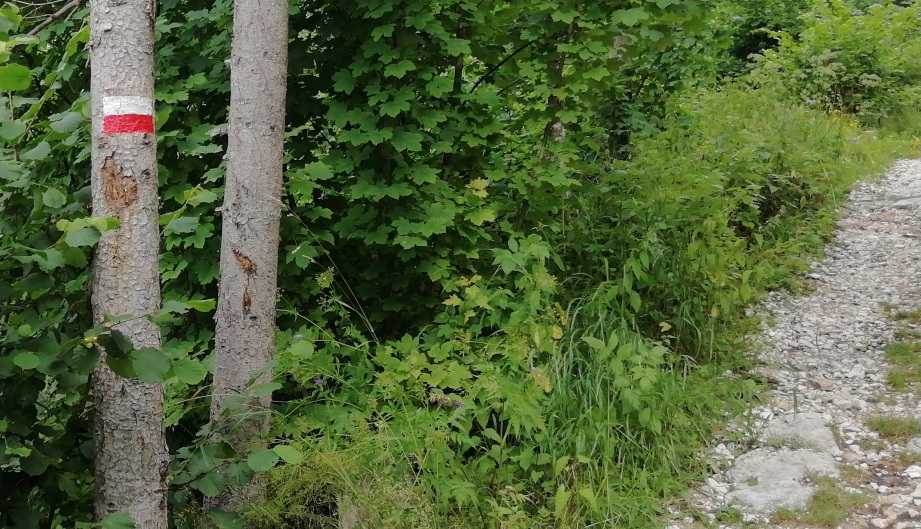
\includegraphics[width = 0.66 \linewidth]{figure/CAI.png}
    \label{fig:CAI}
}
\hfill
\subfloat[A direction sign]{
    \label{fig:pole-direction}
    \includegraphics[width = 0.285 \linewidth]{figure/cartelli.png}
}
\caption{Signs frequently found on trails in Italy}
\label{fig:traditional}
\end{figure}

The functions of signage are twofold
\begin {itemize}
\item an effective signage must guide the tourist across the resort. A map represents a starting point to this end, but not all visitors feel comfortable reading a map. The ideal signage should include visible reference points and explicit actions, like "turn right after crossing the stream". A good example of such signage is the one used by the Italian Alpine Club (CAI), consisting of colored stripes marked on tree bark (see figure \ref{fig:CAI}). The marks are placed in such a way that standing near one of them, the hiker can spot the successive on the trail
\item a sign should explain the reasons for interest in a site. This includes featuring the site where the sign is installed, but also other nearby points of interest that invite the visitor to continue the visit (see figure \ref{fig:pole-direction}). In this sense, the CAI signal above is not useful. A simple board with a site name may be sufficient only when the site is sufficiently popular. Otherwise, a more structured message should be used to explain the reasons why the feature is regarded as relevant.
\end{itemize}

In our study, we consider a range of solutions that help towards sustainable support to sustainable tourism, specifically to the dynamic provision of information during a visit along a natural trail, not covered by Internet connectivity (a {\em dead zone} using the term used by Pearce and Gretzel \cite{pea12a}). We consider the presence of two stakeholders for the signage itself \cite{wan22a}: the hosting organization (the {\em host} for short) which implements a signing installation, and the visitor (or {\em user} ) which extracts useful and enjoyable information from signing devices. 

The purpose of such an installation is guiding the {\em user} on a tour that includes urban streets, buildings, natural trails, and caves (this latter being the topic of the project giving financial support to our research). The task of the {\em host} organization is to provide the {\em user} with all sorts of information that may guide him across the visit, making it as profitable and enjoyable as possible. A traditional approach makes use of physical information boards with graphical or textual content, as in figure \ref{fig:traditional}.

Our study starts by pointing out the issues related to such a solution:

\begin{itemize}
	\item dimensions: the board must be sufficiently large to contain the desired content, taking into account its readability from a distance
	\item installation logistics: depending on the location, the transportation and placement of a plaque may require a basement or other sorts of supports
	\item environmental impact: to be effective, the plaque has to be prominent, and this may negatively affect the quality of the site 
	\item accessibility for the visually impaired: the plaque is not useful for visually impaired persons
	\item accessibility for stranger visitors: to limit the size of the plaque, the number of translations must be limited as well
	\item update limits: to update the content, the plaque must be replaced
	\item removal logistics: when the board degrades it must be either removed or replaced, which entails waste disposal together with other issues similar to those found during the installation
\end{itemize}

Such considerations motivate an interest in an alternative way of communication.

\subsection{Technology to minimize intrusion \label{sec:minimize}}

We characterize the problem as an instance of {\em weak sustainability}: we do not preclude intervention in the environment, but the impact of such intervention must be better than that related to traditional signs. To this end, we include in our solution tools that are not part of the site but remain with the user.   

During the last decades, we witnessed the diffusion of smartphone devices, and we have no reason to expect a change in such a trend. Smartphones empower individual communication capabilities, allowing them to receive sound, visual, and tactile interactions. The relevance of such capabilities for the improvement of a tourist experience has been widely investigated, either in urban environments \cite{liu16a} or in a rural milieu \cite{kum20a} to find ways to exploit such tools. Again, we start from the limits of such technology, especially in the case of outdoor activities.

One is that smartphones although widely available, are not equally familiar to everybody. This is related to {\em usability}, with a term borrowed from P. Wan in \cite{wan22a}. The second is that several functions depend on the provision of enabling services: for instance, their networking capability is useless if the device cannot reach the Internet. So the {\em applicability limits} of a solution need to be defined.

Starting from the two aspects above we envision the guidelines for a successful smartphone-based strategy, keeping in mind its sustainability.

Regarding {\em usability}, the basic recommendation is to keep the operation as simple as possible, within the experience of the majority of users, without requiring the need to familiarize themselves with new applications.

The definition of its {\em applicability limits} is more complex, especially for outdoor activities. In such cases, the provision of a networking infrastructure incurs a severe environmental impact. Consider the installation of antennas to cover a wide area and the power supply for the radios. 

% Circular economy

\subsection{Related works}

The research literature marginally covers the utilization of smartphones for tourist signage purposes.

An exhaustive solution is described by P. Liu in \cite{liu16a}, which details an infrastructure that guides the visitors inside an urban milieu. In that case, the presence of pervasive networking facilities is a cornerstone for the whole architecture, which deeply depends on Internet connectivity. 

Wan \cite{wan22a} evaluates the quality of signage, without referring to a specific technology, but with many examples showing physical boards, using as a formal reference the Universal Design Principles \cite{udi97a}.

The number of research papers explodes when we extend the range to articles investigating smartphones' impact on tourism. The {\em smart tourism} topic is very popular, and covered by several review papers that provide a framework to the vast literature.

A popular research direction covers the social aspects related to the use of the smartphone. W. Tan \cite{tan17a} covers all aspects of a touristic experience related to the smartphone, from the definition of travel destination to assistance during the visit. Much attention is dedicated to the network of connections that is established thanks to the smartphone, which, again, is considered on the Internet. Such an assumption is in contrast with the title, which indicates a nature-based destination, where notably the Internet is not always reachable.

On the other hand, roaming in places not reached by the Internet, or {\em dead zones} using the words of Pearce and Gretzel in \cite{pea12a}, may evoke contrasting feelings, from rewarding to threatening.

More recently, the smartphone has been considered not strictly related to communication. In 2021 A. Slavec et al. investigated the use of cameras \cite{sla21a} while on travel in locations with a relevant cultural heritage to sustain its preservation and engage the tourists using location-based games, similar to Pokemon Go or geo-caching.

In 2023 V. Rodrigues et al. published a systematic review of papers considering the interrelationships between tourism and portable digital devices \cite{rod23a}. Although the title evokes a one-way contribution, i.e., the impact of digitalization is assumed to be positive on the quality and the sustainability of touristic offers, in the conclusions the authors reveal the awareness for the need to address {\em "the preservation of tourism attractions/sites"} and call for a {\em "a holistic approach ... to support a concept that still lacks conceptual and empirical clarification"}.

In that direction, we meet the phenomenon of {\em overtourism}, covered by significant literature reviewed by Dodds and Butler \cite{dod19a}, which focuses on urban tourism and its social consequences. The impact of {\em overtourism} on resorts that trade on their natural resources is investigated in the case of the Hawaii Islands \cite{lin22a} or Costa Rica \cite{mat10a} stressing the impact on the social fabric.

The present paper wants to fill the gap highlighted by Rodriguez, providing a conceptual yet pragmatic approach to a well-defined aspect of tourism support, taking into account "by design" its sustainability. Once a range of relevant solutions has been identified, we proceed to the empirical part: a {\em proof of concept} implementation that verifies the feasibility of a specific solution.

We stress that this article does not aim now at quantifying user satisfaction or the economic revenue associated with the specific solution. Such a target is outside the scope of our research, and indeed the figures that would measure the success of a strategy deserve further investigation. We aim at isolating an issue, proposing a sustainable strategy for its solution, and implementing a proof of concept for it.

\subsection{A simple, low-impact solution}

We aim to design sustainable and effective smartphone-based signage.

A straightforward approach concentrates on the wireless capabilities of such a device. Given the premise that the Internet is not reachable, the {\em host} stakeholder might provide a local network of low-power radios covering the region of interest. Small servers connected to the network would provide specific Web services. The approach requires a modest investment and a marginal environmental impact: for instance, a small device based on the ESP8266 single-chip computer (SCC) has a coverage of tens of meters, and a volume in the order of the $cm^3$. They can provide WiFi Access Points as well as Web content. The ESP8266 has a capacity of 32KB, which is sufficient for explanatory text and a low-resolution image. Other SCCs, like the ESP32, are more powerful but exhibit a higher power consumption. 

Power supply dependency is a serious limitation for such kind of solution. A radio transmitter is a rather power-consuming device, in the range of Watts. Even if intermittent, the operation of a battery-operated networking device cannot be guaranteed for long periods and the host organization should consider power harvesting, which negatively contributes to the economic cost and environmental footprint of the device.

For this reason, we do not consider a solution based on the deployment of a networking facility as a valid competitor against traditional board-based design. As explained, the reasons are related to poor sustainability.

An alternative consists of the utilization of passive devices, like Near Field Communication (NFC) transmitters. The transmitting device is flat, the size of a coin, and costs less than one dollar per piece. To receive the content the smartphone must be very close to the NFC tag. The power needed to operate the radio is drained from the smartphone so that the transmitter does not depend on batteries. The NFC device capacity is in the range of the KBytes, nearly a page on this journal. Storing content in an NFC tag requires a smartphone with a specific app.

The NFC technology is currently very diffused, and reading an NFC tag as text requires the installation of an appropriate application. Once the application is running the operation simply consists in approaching the smartphone to the tag: the tag content is transferred to the {\em user's} device as a chink of text which can be treated as such. The smartphone can read it aloud, to compensate user's inabilities, or translated, to cope with linguistic issues. Such capabilities do not need an Internet connection.

Another solution in the family of passive devices is the QR tag (QR stands for Quick-Response). Such a technology does not require radio communication but uses the smartphone camera to acquire a graphical code that is translated into text. The capacity of a QR tag depends on the number of dots in the image, which in turn depends on the size of the code and the smartphone camera characteristics. We may consider that the capacity of a QR tag roughly equals that of an NFC tag. A QR tag is larger than an NFC tag of comparable capacity, and manufacturing requires a printer.

\begin{figure}
	\centering
	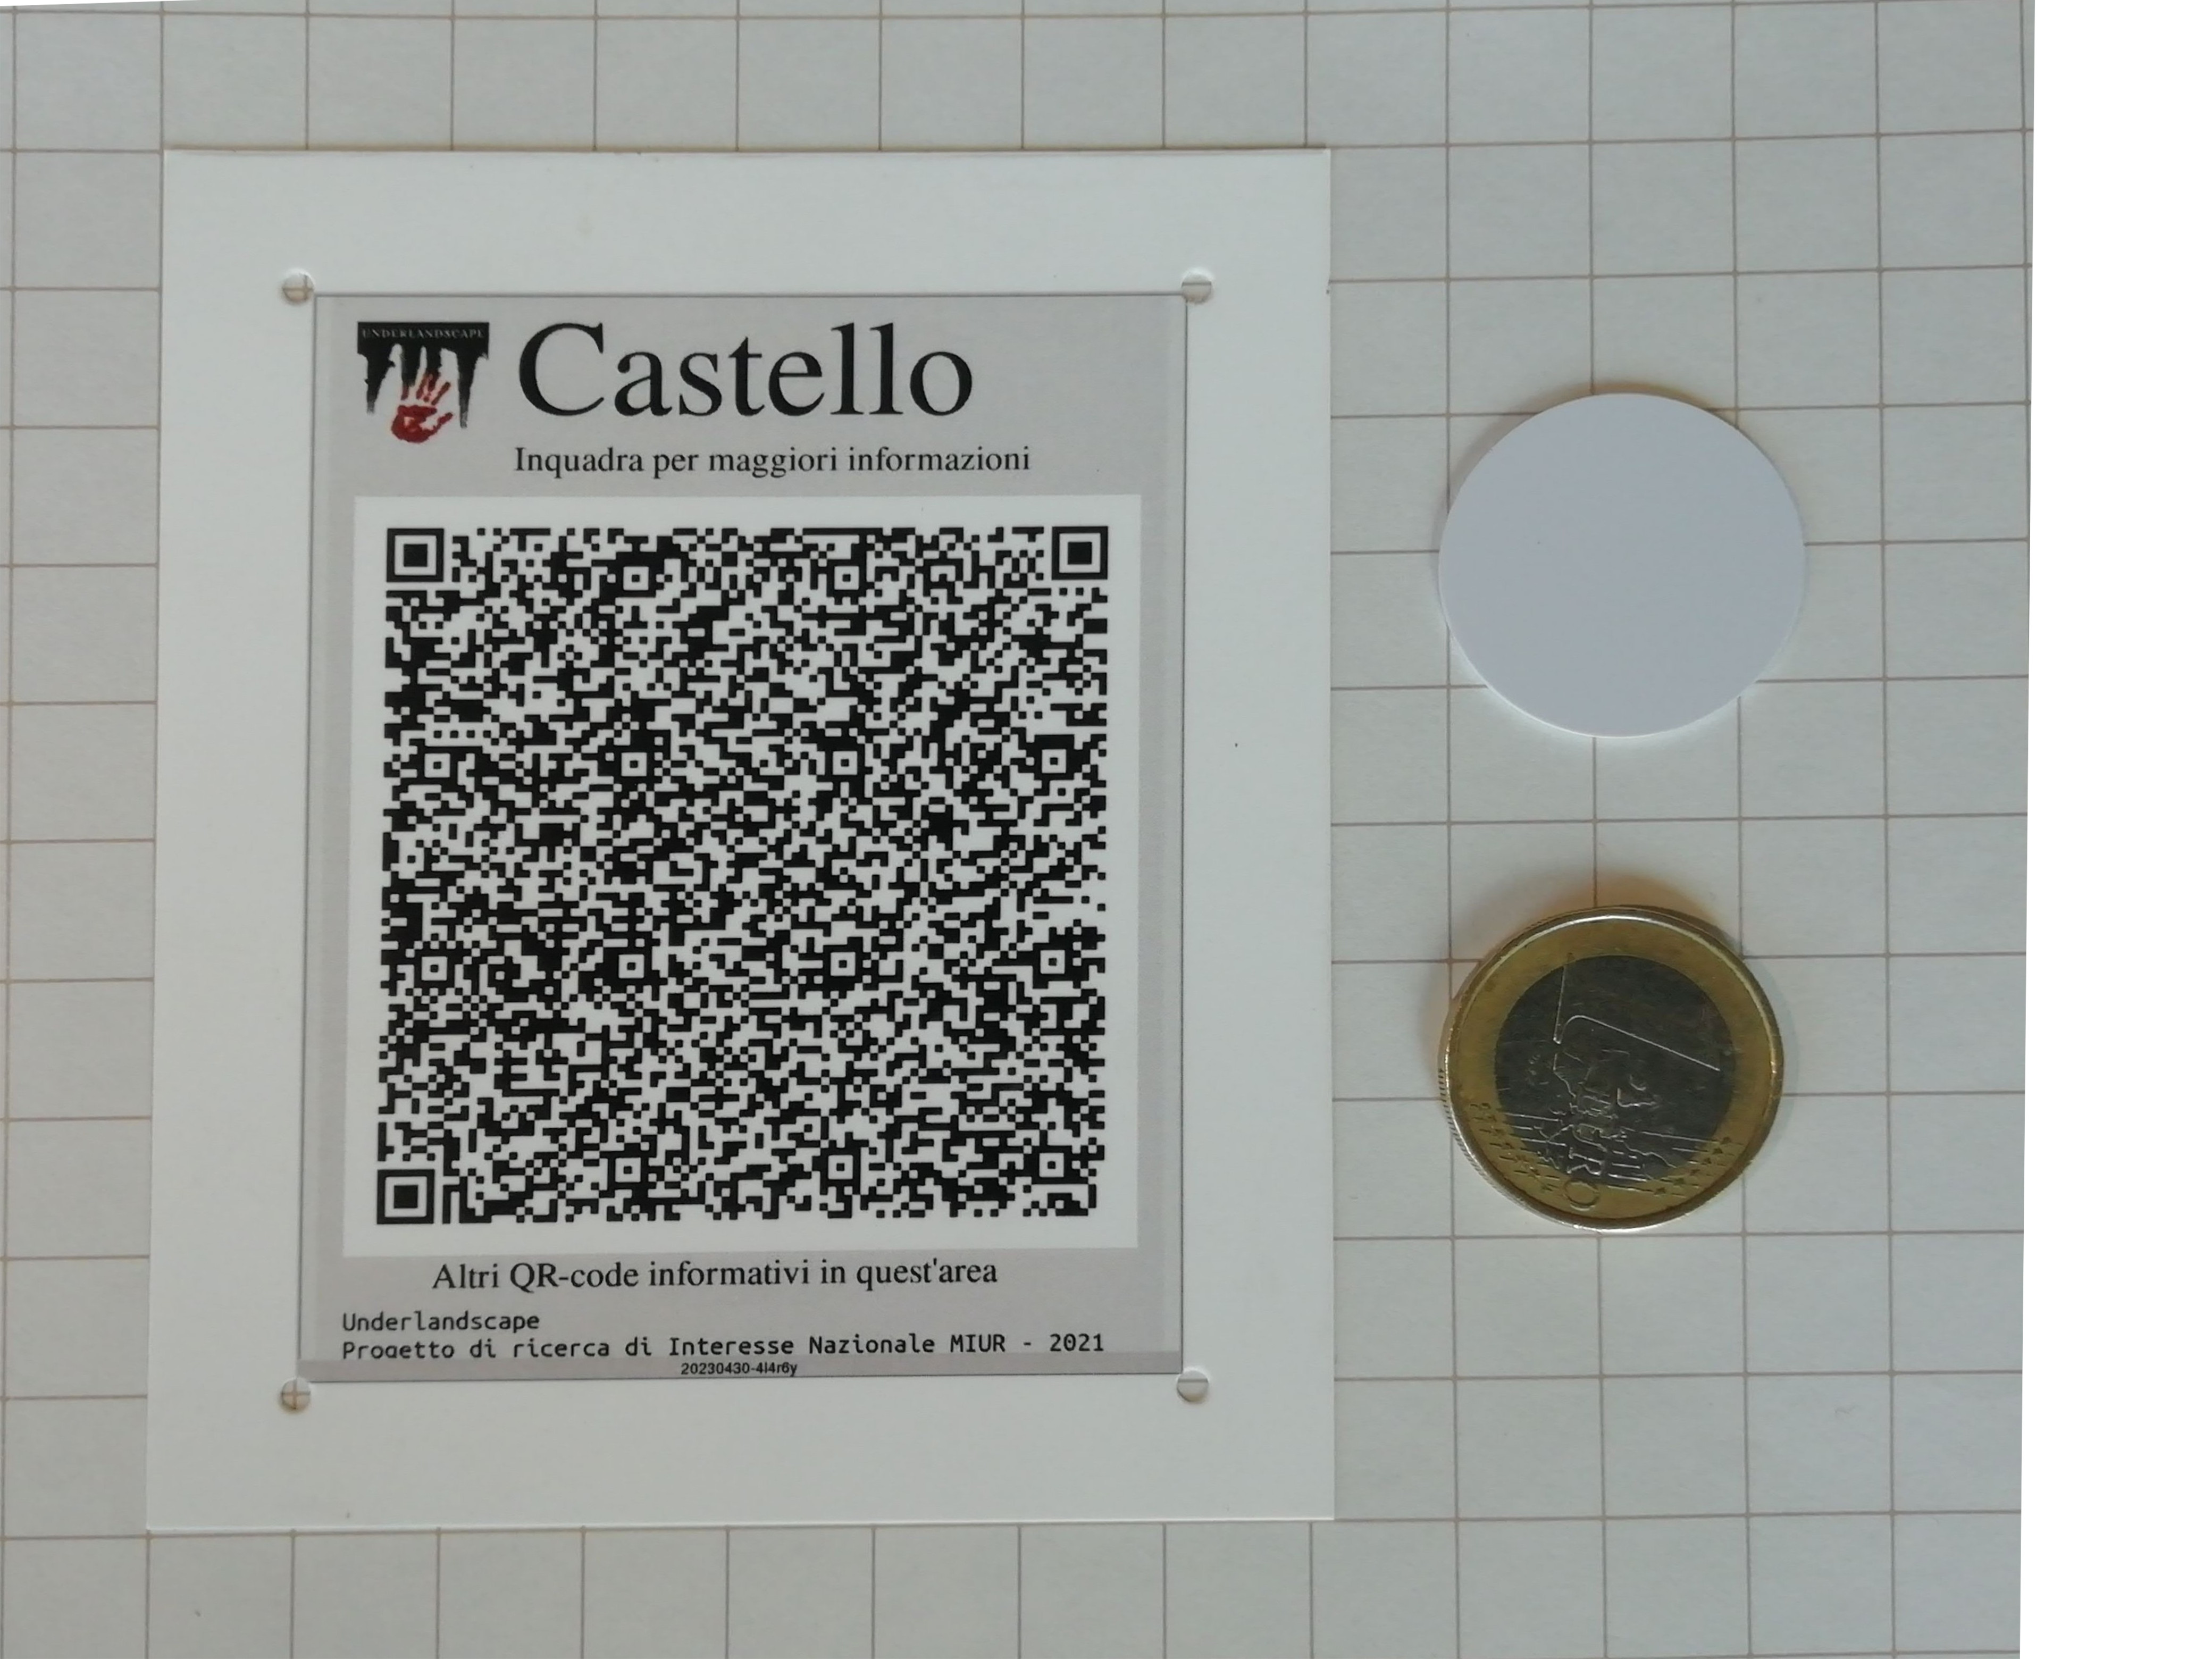
\includegraphics[width=0.9\linewidth]{figure/qr+NFC+coin}
	\caption[Passive devices dimensions]{An NFC coin, a QR tag used in the prototype, and a 1 Euro coin by comparison on a paper with a square of 1cm}
	\label{fig:qrnfccoin}
\end{figure}

A preliminary check verifies compliance with the Universal Design Principles \cite{udi97a}:

\begin{itemize}
	\item {\em Equitable use} is closely related to the smartphone technology, which is itself considered a vehicle for equitability,
	\item {\em Flexibility in use} is enabled by the device capabilities, which allow listening instead of reading, translating the information in a different language, or storing it for later use,
	\item {\em Simple and intuitive use} holds since the operation requires a single application, possibly already installed since useful in many circumstances, and tag reading requires a single finger touch on the smartphone
	\item{\em Perceptible information} is a critical requirement, which contrasts to keep low environmental intrusion. This point will be further discussed in the section devoted to the implementation
	\item{\em Tolerance for error}: there are no margins to use the device in a way that compromises user safety. The deliberate or accidental release of the passive device into the environment determines a minor pollution
	\item{\em Low physical effort} holds, although the user needs to carry the smartphone
	\item{\em Size and Space for approach and use} need to be carefully considered. In the case of the NFC tag the smartphone needs to be nearly in touch with the passive device, while the QR code must be in the line of sight and frameable without effort
\end{itemize}

Such minimal solutions (see figure \ref{fig:qrnfccoin}) compare well with other more complex ones that make use of the user's smartphone. There is a trade-off concerning capacity, but in many circumstances, a capacity of 2-300 words is sufficient to convey the description of the site or provide directions for the visit. If capacity limits are not an issue, a solution based on NFC or QR tags exhibits several advantages:

\begin{itemize} 
\item does not require any power supply,
\item has a limited impact on the landscape,
\item does not entice theft,
\item has a negligible cost,
\item is durable,
\item produces a limited quantity of waste when disposed of,
\item content can be stored for later usage; for instance, to visit a URL once the user reaches a zone covered by the Internet.
\end{itemize}

The two passive technologies of choice exhibit the following features, that may make one of them preferable for a specific application:

\begin{itemize}
	\item an NFC tag is smaller than a QR tag;
	\item writing an NFC tag requires a smartphone, while the QR tag needs a printer;
	\item reading an NFC tag works near-to-contact, while QR tags can be read from a distance;
\end{itemize}

%It significantly outperforms any active device, except for the capacity, and the NFC compares favorably only when capacity and size are prominent.

For a signage application, a QR tag is preferable because a noticeable size is needed. In addition, keeping the tag out of reach prevents vandalism and misuse.  

In conclusion, we have reasons to select a QR-tag-based solution as a good candidate for smartphone-based signage. We now consider how it copes with the limits of a traditional board-based approach (as listed in table \ref{sec:signage}):

\begin{itemize}
	\item dimensions: a 2-300 characters QR-code has a dimension in the order of 100 $cm^2$
	\item logistics: QR-code board can be installed on any sort of pre-existent or natural support
	\item impact: the board has minimal interference with the landscape and may easily go unnoticed
	\item accessibility for the visually impaired: the text can be read aloud
	\item international: the text can be translated automatically
	\item update: the board can be easily replaced when the content becomes obsolete
	\item disposal: the card releases a limited quantity of pollutants related to ink support (paper or plastic)
\end{itemize}
		
There are two relevant trade-offs that the host needs to resolve. One is related to the visibility of the tag. The trade-off is between visual impact and visibility. The other is related to monitoring tag utilization. This may be useful for all sorts of planning activities and is discussed in section \ref{sec:results}.

\section{Materials and Methods}

As anticipated in the introduction, our study wants to provide a proof of concept for a sustainable solution in a concrete setup. To comply with such a holistic approach, we need to start with the definition of the operation framework.

This section is devoted to the description of an economic and social context, as well as the historical background representing the heritage resource we want to promote. Next, we will discuss the technical details of the solution.

The geographical area of interest is the surroundings of \emph{Casoli}, a small village in a mountainous region in the north of Tuscany, in Italy. The area falls within the municipality of \emph{Bagni di Lucca}, in the province of \emph{Lucca}. In 2021, the archaeological team of our project realized an archaeological map assessing the reasons of interest for the heritage and the geomorphological features of the area.

\subsection{The natural and cultural resources of \emph{Casoli} and its vicinity}

\emph{Bagni di Lucca} is located on the north-eastern boundary of the Province of \emph{Lucca}, in \emph{Val di Lima}, and is part of the \textit{Media Valle del Serchio} district. With its mountains it marks the historical border with the Modena and Pistoia area, it is very rich in potential for its naturalistic, archaeological, and historical heritage, both expressed and as yet unexpressed. Thanks to the archaeological map the main sites of interest from prehistoric to contemporary times in this municipality are cataloged, photographed, and georeferenced.

From a historical-geographical point of view, this area is identified with the \emph{Lima} stream and its tributaries, which impress to the area a particular geomorphology, very impervious despite the modest hilly elevations.

The \emph{Lima} stream has characterized the history of \emph{Bagni di Lucca} since ever: some of the oldest evidence of human presence in the valley has been found along its ancient river terraces, such as caves and rock shelters frequented since the Palaeolithic age; the manufacturing industry (paper mill, flour mills and, in recent times, energy production) have exploited since the Middle Age until the 1980s \cite{men76, bed05, ser21}.
 
On the naturalistic side, the region of \emph{Bagni di Lucca} encompasses an incredible concentration of biodiversity, counting no less than three sites of the Natura 2000 Network \cite{nat00} European Economic Community (EEC) initiative.

There are three SCIs-SACs (Sites of Community Interest and Special Areas of Conservation) located in the area north of the \emph{Lima} stream, corresponding to the Apennine portion, covering 23\% of the municipal surface:
\begin {itemize}
\item the limestone areas of \emph{Val di Lima} and Balzo Nero; 
\item Monte Prato Fiorito-Monte Coronato-Valle dello
Scesta; 
\item Orrido di Botri.
\end{itemize}

%\begin{figure}
%	\centering
%	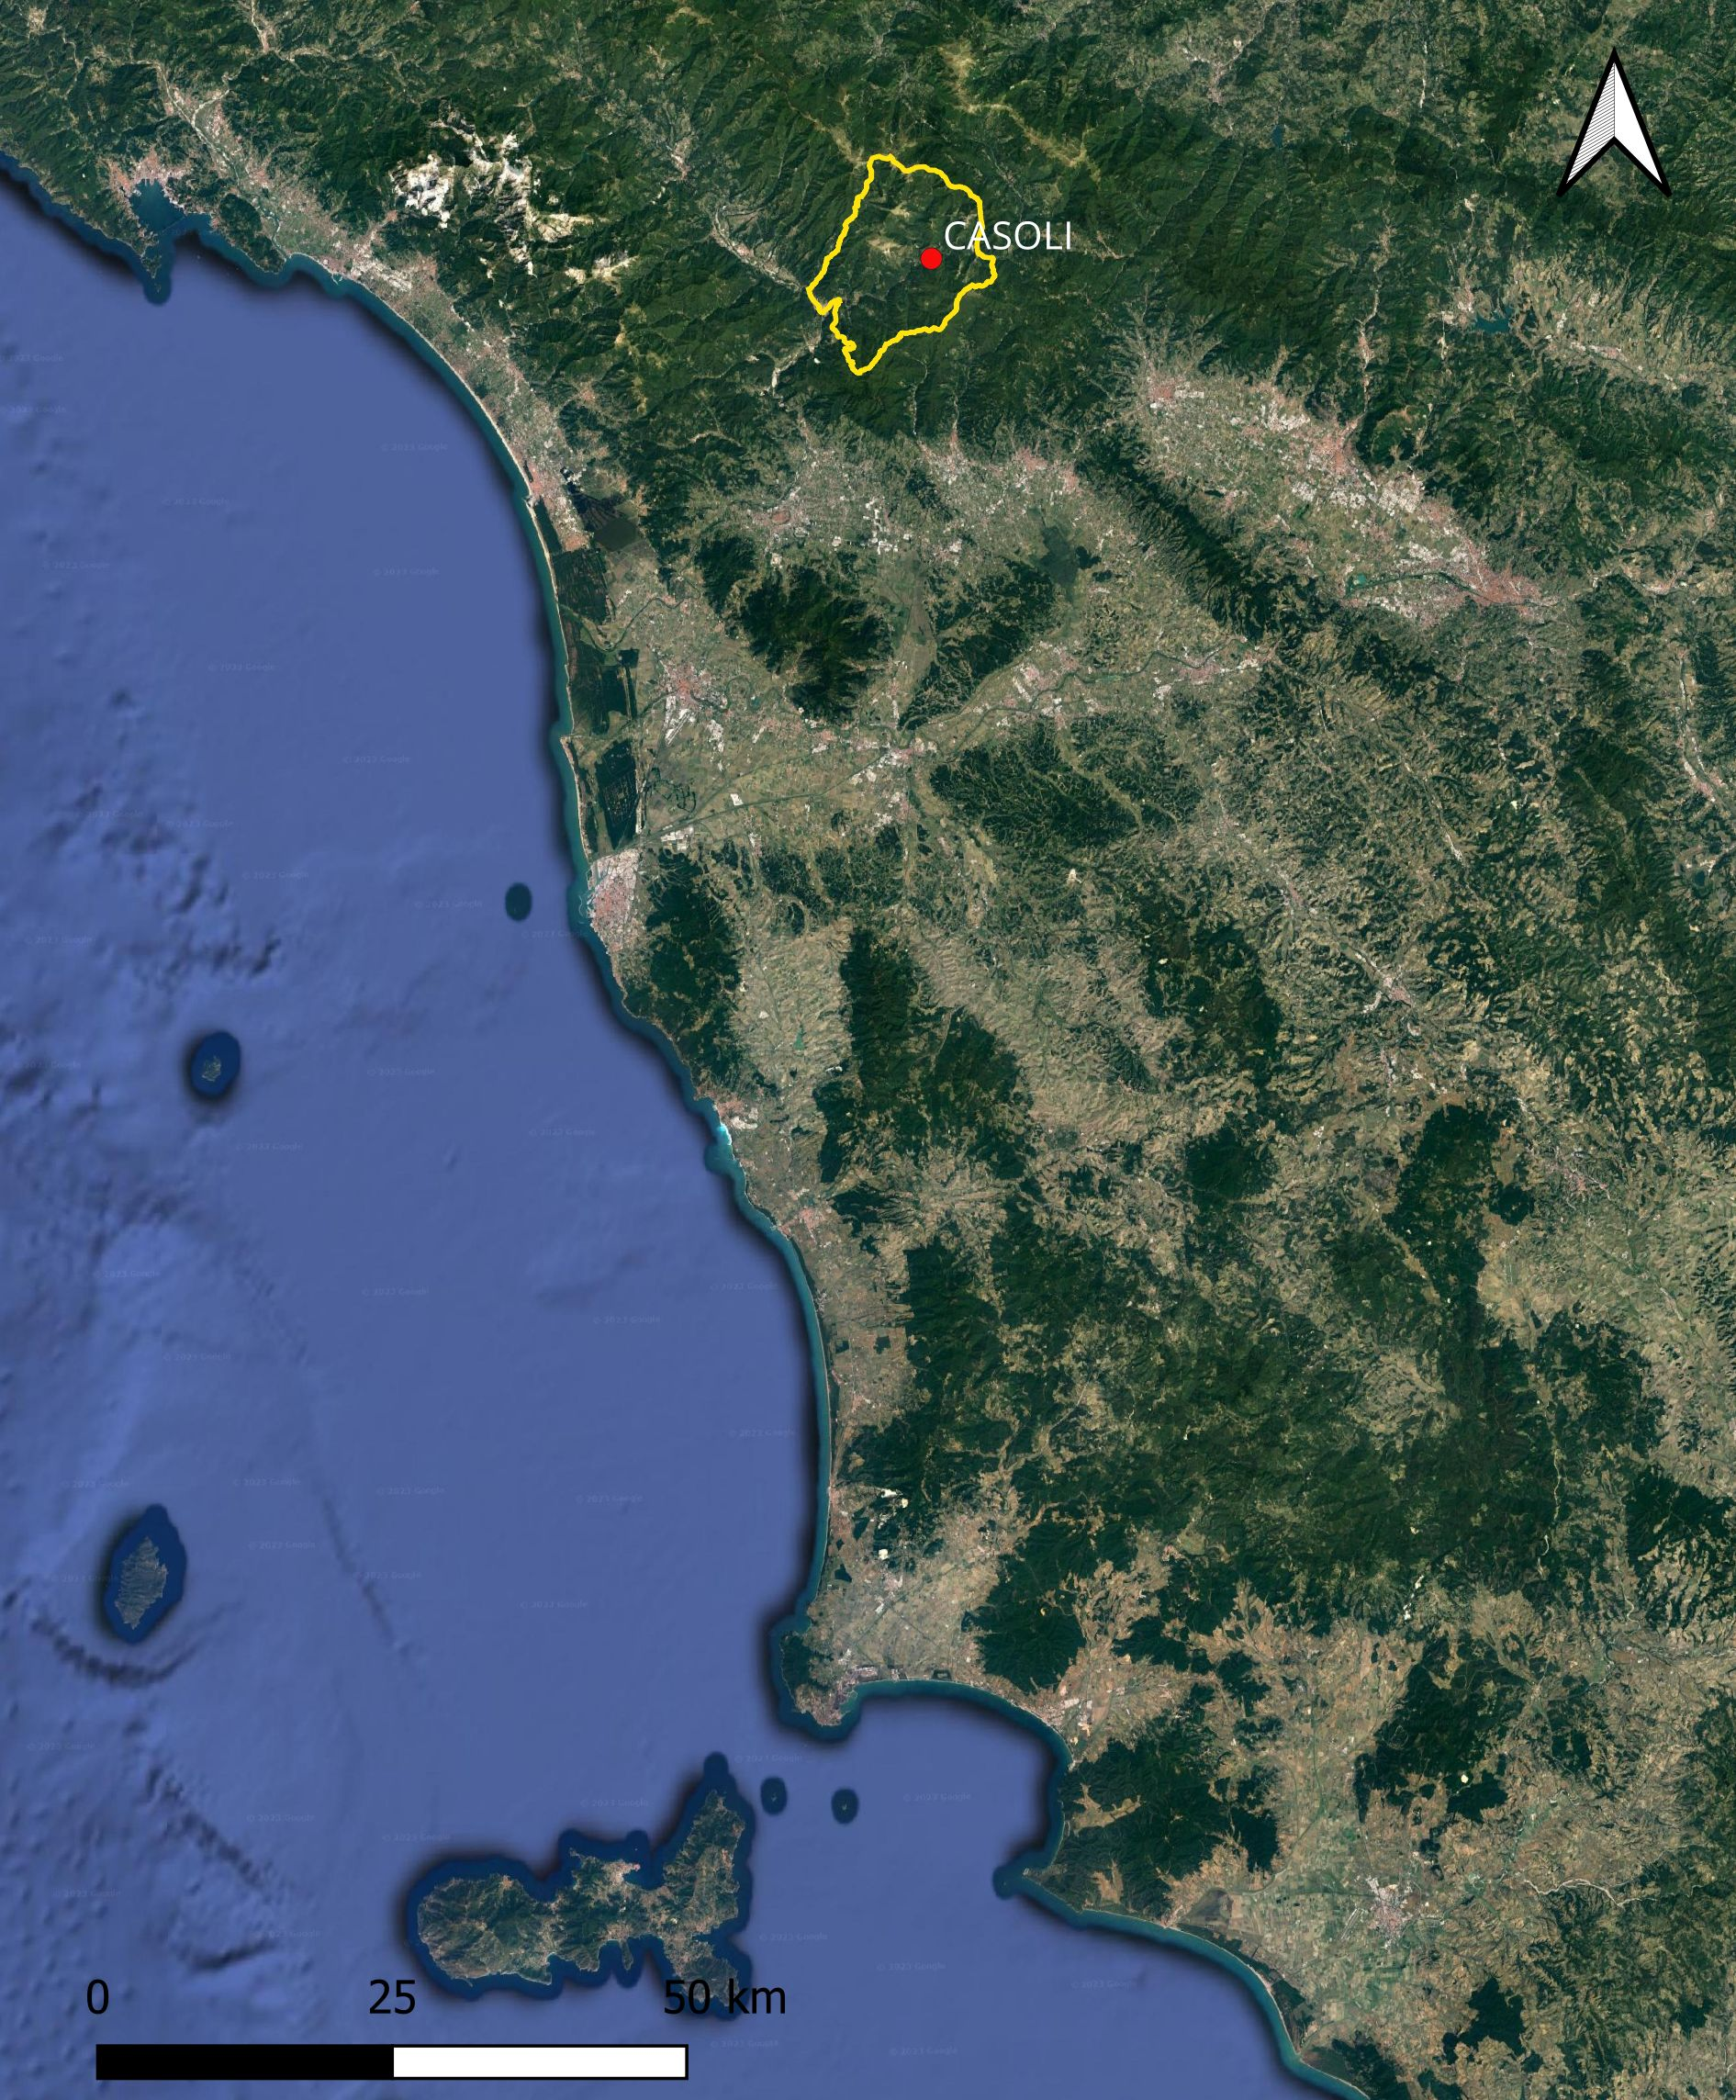
\includegraphics[width=0.3\linewidth]{figure/toscana-casoli}
%\end{figure}

\begin{figure}
\subfloat[Italy and Tuscany, bordered in red]{
	\includegraphics[width = 0.3\linewidth]{figure/italia.png}
	\label{fig:population}
}
\hfill
\subfloat[Tuscany and the municipality of \emph{Bagni di Lucca} (in yellow)]{
	\includegraphics[width = 0.3 \linewidth]{figure/toscana.png}
	\label{fig:tourismflows}
}
\hfill
\subfloat[Location of the \emph{Casoli}  village in the \emph{Bagni di Lucca} municipality, bordered in yellow. The small town of \emph{Bagni di Lucca} is visible located a few kilometers west of \emph{Casoli} ]{
	\includegraphics[width = 0.3 \linewidth]{figure/bagni_di_lucca.png}
	\label{fig:tourismflows}
}
\caption[The region of \emph{Casoli}]{The region of \emph{Casoli}}
\label{fig:toscana-casoli}
\end{figure}

The latter is also a SPA (Special Protection Area) and the \textit{Orrido di Botri} State Reserve is located within it \cite{nat00}. It is therefore a natural heritage with a fragile balance that needs to be preserved.

In recent years, the main tourist attractions have concentrated on the \emph{Lima} stream, with some associations and private entities promoting outdoor experiences, particularly fluvial sports, such as canyoning, rafting, and sup. Other important tourist attractions are trekking and hiking, supported by a network of paths tracked by local CAI (\textit{Club Alpino Italiano}).

In the last few years the community opened two entirely new trails:
\begin{itemize}
	\item the \textit{Alta Via dei Pastori} (2019), a ring around \textit{Monte Prato Fiorito} that takes up the ancient grazing route, and
	\item the \textit{Sentiero degli Avi} (2020), a ring that from \textit{Montefegatesi}
	reaches \textit{Monte Coronato} \cite{pin21}
\end{itemize}

Another recently developed project (2019) is the expansion of the Saint Bartholomew's Path, which runs through the territory of \textit{Pistoia}, with a
variant that from \textit{Popiglio} continues in five stages in the municipality of \emph{Bagni di Lucca} to \textit{Pieve di Controne}, acting as the '\emph{Lucca} gateway' to the Path \cite{camsb}.

Such initiatives led to a considerable revival of interest among Italian and international hikers in the area, especially for the Apennine side of the valley.

The way to improve the valorization and enjoyment of this area applies to a slow tourism approach. This approach can involve the community, especially in the southern part of the municipality, which is still less frequented, more hilly, and therefore less traveled by the network of trails. We propose the creation of geo-itineraries characterized by the rediscovery of the historical roads, partly well-preserved, which connected the villages with the valley bottom and between them, including those sites of interest that encapsulate the history of this area, starting with the caves.

\subsubsection{An historical perspective of an Italian mountain site}

 The village of \emph{Casoli} is located south of the \emph{Lima} stream on a hill named {\em "Tanette"}. In the local small lair, the name reveals the presence of karstic cavities, some inhabited between the Paleolithic and the Iron Age and used also as stations on the trans-Apennine routes \cite{men76, gia96, pal63, zec72a, zec72b}.

Ceramic fragments dated between the 3rd century B.C. and the 1st-2nd century A.D. prove that Ligurian populations occupied the region scattered and in small nuclei. The dedication of the Latin colony of \textit{Lucca} in 180 B.C. marked a decisive turning point in the Romanisation of the area and, shortly after, the definitive subjugation of the Ligurian populations, accompanied by a rapid acculturation \cite{gia96, cia05}.

We have little evidence of Roman settlements in the mountainous hinterland, and the scarce archaeological traces are concentrated in the cave of \textit{Buca La Piella}, investigated in 1975 by the Centre for Archaeological Studies of \emph{Lucca}; it has two entrances joined by a walkable tunnel and rooms of discrete dimensions that overlook the outside. In addition to numerous faunal remains and fragments of locally produced common pottery, twenty bronze coins belonging to the 3rd century AD, bronze and lead objects were found \cite{gia96, men81, cia03}. 

In Longobard and Carolingian times, \emph{Lucca}'s \emph{Val di Lima} was one of the three administrative districts into which the mountains were divided and was called “fines Contronenses” \cite{qui02, cia06, cia11}. The only find from this period is the \textit{Grotta di Arzale}, a rock shelter that opens up northwest of \emph{Casoli} \cite{gia96}.

The first attestation of the settlements of \emph{Casoli} and \emph{Lacu} (Lake) dates back to the 10th century \cite{gia96}. Most documents of this period show the fractioning and alienation of ecclesiastical heritage in favor of the city aristocracy, securing an accumulation of funds and power that was to form the basis of the subsequent domains \cite{qui02, gia96, for12, for15}.

Written sources mention a castle in \emph{Casoli} from 1180, but its foundation must be earlier. Between the 13th and 15th centuries, the fortification was at the center, along with the other castles of the \emph{Val di Lima}, of clashes between \emph{Lucca}, \textit{Pisa} and Florence, with alternating fortunes, as it was a strategic border area for the power of \emph{Lucca}. Today, very little is preserved and the area has been partly inhabited \cite{gia96, for12, rom16}.

The same document from 1180 mentions the church of \textit{San Donato}, located in the main square of the village of \emph{Casoli}. The current structure dates back to the 12th-13th centuries, with subsequent renovations. Initially dedicated only to \textit{San Donato}, it acquired a double dedication after the abandonment of the church of \textit{Sant'Andrea de Lacu}. The latter is located on a plateau to the east of Lake \emph{Casoli} and is attested from 1260 \cite{ber18, gia96, cap17}, but already in the 15th century, we learn of its state of abandonment \cite{gia96, con12}. This was probably due to the depopulation of the lake area and the simultaneous strengthening of the town of \emph{Casoli}, which was fortified and better protected during this unstable phase.

Today, the Romanesque church of \textit{Sant'Andrea de Lacu} is in a state of decay, with a rectangular plan, ending on the east side with a semi-circular apse. Inside, there is a reused element of the previous building, testifying to an older origin, probably contemporary with the ancient settlement of \textit{Lacu} (Lake) mentioned in sources from the 10th century and no longer visible today.

In the early modern age, villages of the area experienced a progressive architectural renewal, which still largely characterizes the settlements today. Within \emph{Casoli}, a series of residential buildings with imposing dated portals are preserved, some with courtyards, and mansions that denote a discrete deployment of resources by wealthy social classes. Also dating from the modern era is the \textit{Madonna di Castello} Oratory, characterized by an entrance enclosure and located along the cobbled road that traces the ancient route between the village and the summit area of the medieval castle \cite{gia96}.

Along the road that led toward \textit{Lucchio} crossing the area of \emph{Casoli} Lake, there is the chapel of \textit{Madonna di Col di Piano} and two “\textit{metati}”, buildings destined for chestnuts drying, referable to the contemporary age. Referred to as the "bread tree," chestnut fruits and the flour derived from them were a staple of the mountain diet until the mid-1900s \cite{buc92, puc10}.


\subsection{An integrated view of tourism in the \emph{Casoli} region}

%\subsubsection{Study of the tourist context for governance approaches}

Within the paper's aim framework and from a touristic point of view, the relevance of the touristic context of the territory is crucial in understanding the socio-cultural system of potential tourist destinations. In light of this and for a holistic study approach to social features of tourism, the host and traveler relationship is directly related to local development and local government systems \cite{amo21}.

In this study, the holistic perception of local stakeholders and community empowerment (with its increasing potential) in tourism at the local level acquires a particular value. For this specific purpose, this paragraph is well related to the tourism dynamics of the Municipality of \emph{Bagni di Lucca}, the administrative land hosting \emph{Casoli}. 

\subsubsection{The tourism context of / The tourist dynamics in \emph{Bagni di Lucca}, the \emph{Val di Lima} and \emph{Casoli}}

In Italy, a municipality is the smallest geographical-administrative unit offering accessible data about tourism, which are the fundamentals of our research. The municipality of \emph{Bagni di Lucca} boasts historical popularity for its landscapes told by famous poets (such as Giosuè Carducci, Giovanni Pascoli, Eugenio Montale, George Gordon Byron, Percy Bysshe Shelley) and celebrities like Paolina Bonaparte. The typical Liberty style architecture characterizes the villas like the \textit{Real Casinò} featuring elegant gardens representing the power of the Republic of \emph{Lucca} in the early XIX century and the \emph{Belle Epoque}. Such historical prominence made the town a well-known destination abroad, thanks to the massive emigration and the presence of the Thermal Bath structure \footnote{Terme di Bagni di Lucca: \url{https://www.termebagnidilucca.it/}}, nearby must-see attractions of the time.

\emph{Bagni di Lucca} owes part of its charm to the river \emph{Lima}, which runs along the city before flowing into the \textit{Serchio} River. The \emph{Lima} Valley (\emph {Val di Lima} in the local idiom) is a touristic basin set in the \textit{Serchio} Valley, dotted with medieval and Roman villages with historical remains such as underground caves. The \emph{Val di Lima} area is well-known for its environmental beauties including rupestrian and lake ecosystems, and offers a wide range of tourist attractions related to sports, from water sports, such as canyoning and rafting, to trekking in water and land, climbing, mountain biking, and horseback riding. Overall, the \emph{Val di Lima} has the capabilities to promote a very identifying destination brand straddling the town of Lucca and the mountain area of the \textit{Garfagnana}.

The strategic position of \emph{Bagni di Lucca} is one of the strengths of its tourism context, together with the presence of such attractive elements like the \emph{Orrido di Botri} with the \emph{Canyon Park\footnote{\url{ https://www.canyonpark.it/}}}, and other service companies and associations for experiential tourism.

The demographic trend enlightens a relevant aspect of \emph{Bagni di Lucca} society, and the employment statistics of the population mirror the social, cultural, and economic aspects of its touristic ecosystem.

\begin{figure}
\subfloat[Population trend (2001-2022)]{
	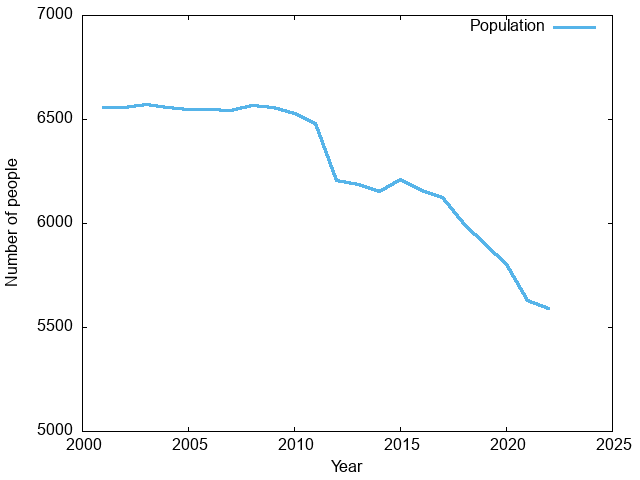
\includegraphics[width = 0.5\linewidth]{figure/population.png}
	\label{fig:population}
}
\hfill
\subfloat[Tourism flows and population (2017-2022)]{
	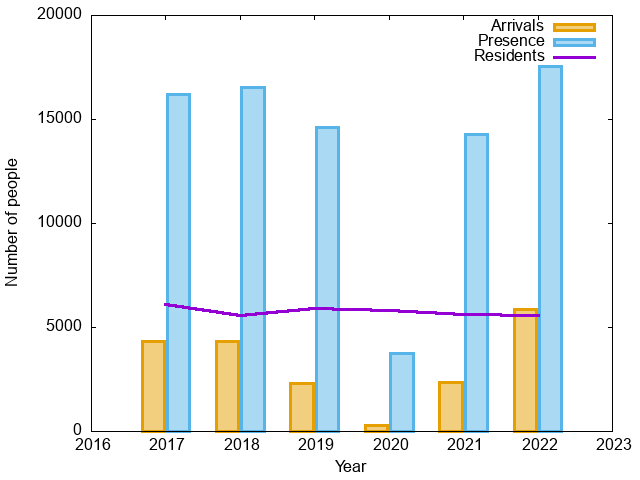
\includegraphics[width = 0.5 \linewidth]{figure/tourism.png}
	\label{fig:tourismflows}
}
\caption{Demography and tourist flows in the municipality of \emph{Bagni di Lucca}}
\end{figure}

%\begin{figure}
%    \centering
%    \includegraphics[width=0.75\linewidth]{figure/Population.png}
%    \caption{\emph{Bagni di Lucca}’s population trend, 2001-2022}
%    \label{fig:population}
%\end{figure}

\emph{Bagni di Lucca} stretches on 164.70 $km^2$ area with a population density \footnote{Index referring to the number of people living in a territory per square kilometer. It is the rate between the annual number of residents and the surface area. In our case and for 2022, the density is 5593 people over 164.70 $km^2$.} of 3395 inhabitants per square kilometer and a job occupancy rate of 33.53\%. Regarding human growth at the territorial level, it is relevant to consider the \emph{Bagni di Lucca} population trend during the 2001-2022 period. The curve shown by figure \ref{fig:population} registers a constant and slight decrease of one thousand people in a twenty-year time frame (2001: 6556 people; 2022: 5593 people). 

During the latest decades, numerous touristic operators have started their touristic activities by taking advantage of the climatic and morphological characteristics of the territory. From a quantitative perspective, it is relevant to understand the tourist flows during a 5-year time frame; the chart in figure \ref{fig:tourismflows} highlights a decreasing trend from 2017 to 2021 by considering the pandemic breakdown impacts on tourism.

%\begin{figure}
%    \centering
%    \includegraphics[width=0.75\linewidth]{figure/TourismFlows.png}
%    \caption{\emph{Bagni di Lucca's} tourism flows, 2017-2022}
%    \label{fig:tourismflows}
%\end{figure}


The Tourism Density Index \footnote{The Tourism Density Index shows the tourism concentration in the higher touristic season. It is the rate between the number of tourists and the surface area.} is 106.41 tourists per $km^2$ in 2022. The arrivals exhibit a drop from 2019 (from  4339 in 2017 to 2363 in 2021), and touristic presences have suffered a slight decrease during the same period, as shown in figure \ref{fig:tourismflows}, while a further increase has been registered in 2022 (5.876 arrivals).

The touristic area of \emph{Val di Lima} features a tourist area belonging to \emph{Bagni di Lucca} Municipality, the second touristic area after \textit{Barga}, in the \textit{Media Valle del Serchio Area}.


%\begin{table}
%    \footnotesize
%    \setstretch{1,4}
%    \centering
%    \begin{tabular}{|c|c|c|c|c|} \hline 
%         Region & Touristic Density & Average stay &  Accommodation density & Coexistence Index\\
%           & (visitors/{$km^2$}) & (days) & (accommodations/{$km^2$}) & (100 $\times$ foreign/italian)\\ \hline
%         Bagni di Lucca & 106,41 &  2,98 &  10,14 & 103,74\%\\ \hline
%         Lucca & 1866,96 & 3,36 & 19,30 & 69,87\%\\ \hline
%    \end{tabular}
%    \caption{Tourist numbers in \emph{Bagni di Lucca} in 2022\tablefootnote{Each  index gives a different type of touristic information about \emph{Bagni di Lucca} Municipality: the touristic density represents the number of tourists per $km^2$; the Average stay index is the average number of nights spent in town by tourists; the Accommodation Density Index is related to the number of touristic presences on the number of beds occupied by tourists all over the year; the coexistence index shows the relevance of foreign tourists per 100 Italian tourists.}}
%    \label{tab:tourism}
%\end{table}

\begin{table}
    \footnotesize
    \setstretch{1,2}
    \centering
    \begin{tabular}{l||l|l} \hline 
        {\bf Region} & {\bf Bagni di Lucca} & {\bf Lucca} \\ \hline
        Resident density (residents/{$km^2$}) & 33.95 & 215.71 \\
        Touristic density (visitors/{$km^2$}) & 106.41 & 1866.96 \\
        Average stay  (days) &  2.98 &  3.36 \\
        Accommodation density (accommodations/{$km^2$}) & 10.14 & 19.30 \\
        Coexistence Index (100 $\times$ Foreign/Italian) & 103.74\% &  69.87\% \\ 
         \hline
    \end{tabular}
    \caption{Tourist numbers in \emph{Bagni di Lucca} in 2022\tablefootnote{Each index gives a different type of touristic information about \emph{Bagni di Lucca} Municipality: the touristic density represents the number of tourists per $km^2$; the Average stay index is the average number of nights spent in town by tourists; the Accommodation Density Index is related to the number of touristic presences on the number of beds occupied by tourists all over the year; the coexistence index shows the relevance of foreign tourists per 100 Italian tourists.}}
    \label{tab:tourism}
\end{table}

Table \ref{tab:tourism} provides statistical data concerning tourist flows and accommodation in \emph{Bagni di Lucca}. Notably, the tourist density of 106.41 tourists per $km^2$ is higher than the population density (33.95 inhabitants per $km^2$).

The number of nights per tourist amounts to an average of 2,98 nights per tourist during a year and it is also significant since it shows, on one hand, \emph{Bagni di Lucca} context appeal for tourists choosing to stay a number of nights more than a weekend and less then a week. On the other hands, this data means that people like staying in this touristic comprehensory and they may have founded attractions, services and activities they need. Consequently, a well-organized turistic system attracts potentially touristic presences widespread on the municipality territory.

The coexistence index describes the distribution of tourist nationalities: 103.74 foreign tourists per 100 Italians in \emph{Bagni di Lucca} indicates a significant share of foreign tourists.

For a benchmarking point of view, the provincial touristic context of \emph{Lucca} is mentioned in this study with the purpose to highlight the percentage weight of \emph{Bagni di Lucca} tourism flows within the whole tourism dynamics of the Province of \emph{Lucca}. 
As concerns tourist indexes shown in Chart 3, the touristic density counts 1866, 96 people per square kilometer (1773 kmq), with an average stay of 3,36 nights per tourist, showing a medium-length permanence in the provincial territory; this data is in line with \emph{Bagni di Lucca} average stay (2,98 nights). 
The provincial area of \emph{Lucca} shows an accommodation density of 19,30 on 10, 14 of \emph{Bagni di Lucca}, while the coexistence index of \emph{Lucca} (with 69,87 foreign tourists on 100 Italian tourists) is lower than \emph{Bagni di Lucca}’s coexistence index (with 103,74 foreign tourists in 100 Italian tourists). 
Definitely, it can be claimed that \emph{Bagni di Lucca} is well positioned in the whole touristic context of \emph{Lucca} since it represents one of the less populated municipalities in the territory with interesting tourist indexes. In fact, \emph{Bagni di Lucca} boasts its historical thermal tourism tradition together with a well-equipped environment for sport and adventure tourism, on a surface of 164,70 kmq, that is one of the biggest municipality areas in the province of \emph{Lucca}.

Summing up, the quantitative data give evidence of a vibrant and attractive tourist reality constantly attracting tourists during the last decade. Thanks to such tourist flows \emph{Bagni di Lucca} is considered one of the main tourist areas of the \emph{Val di Lima} and the Serchio Valley. Several promotional websites advertise \emph{Bagni di Lucca} attractions\footnote{Among local websites, these two destination websites are: \url{www.turismobagnidilucca.com} and \url{www.valdilima.org}}: the sitography closing this paper contains a long but incomplete list that confirms such a statement, and Table \ref{tab:experience} exposes the promotional touristic system offering varied experiences in the \emph{Val di Lima} area. The variety of outdoor touristic services dates back to the ‘90s when some associations began organizing mainly trekking excursions and rafting experiences.

From the point of view of our research, the context of the \emph{Bagni di Lucca} helps to understand the complexity and variety of mixed tourism clusters (a sort of "touristic ecosystems" with common identitary elements such as: anthropic, socio-cultural, and historical features, as well touristic services).

After a detailed analysis of the touristic and social context of \emph{Bagni di Lucca}, it can be claimed that the area boasts a good tourist appeal towards Italian and foreign tourists searching for various kinds of experiences, such as thermal, environmental, outdoor, sport and cultural activities  \cite{loz09}.

%Indeed, \emph{Val di Lima} can promote a very identifying destination brand straddling the town of Lucca and the Garfagnana mountain area. The strategic position of \emph{Bagni di Lucca} is one of the strengths of its tourism context, together with the presence of such attractive elements like Orrido di Botri, with The Canyon Park \footnote{\url{ https://www.canyonpark.it/}}, and other service companies and associations for experiential tourism.

\begin{table}
    \centering
    \begin{tabular}{|p{70mm}||p{45mm}|} \hline 
         {\bf Touristic promotion }&  {\bf Kind of service}\\
         \hline \hline 
         Aguarajà River Experience \newline \url{https://aguaraja.it/}& Soft rafting, Rafting, Canyoning, aqua-trekking, kayak\\
         \hline 
         Rafting H2O \newline \url{https://www.raftingh2o.com/}& Soft rafting, Rafting, Canyoning, aqua-trekking, kayak\\
         \hline 
         RocKonda \newline \url{https://www.rockonda.it/}& Soft rafting, Rafting, Canyoning, aqua-trekking, kayak\\ \hline 
         A.S.D. Garfagnana Rafting \newline \url{https://www.garfagnanarafting.com/}& Soft rafting, Rafting, Canyoning, aqua-trekking, kayak\\ 
        \hline 
         Val di Lima Off-Road \newline \url{https://www.valdilimaoffroad.com} & Quad, enduro\\ \hline 
         Canyon Park \newline \url{https://www.canyonpark.it/canyon-sup}& Canyoning, aqua-trekking, stand-up padding, mental care and yoga, eco laboratory\\
         \hline 
         Pro Loco Bagni di Lucca \newline  \url{https://www.turismobagnidilucca.com/} \newline \url{https://www.valdilima.org/}& Sportfishing, mental care, trekking, survival, paragliding, horse riding, diving\\
         \hline 
         eBike Adventure Tour \newline \url{http://www.ebikeadventuretour.it/}& Ebike, Mountain bike\\ \hline 
         Val di Lima eBike \newline  \url{https://valdilimaebike.it/} & Mountain e-bike, Quad, Enduro, Paintball\\
         \hline 
        Terme Bagni di Lucca \newline \url{https://www.termebagnidilucca.it/} &Spa, beauty and wellness experience\\
        \hline
    \end{tabular}
    \caption{\textbf{Tourism experiences’ offer in \emph{Val di Lima} area \tablefootnote{The list might not include all private stakeholders of the territory, since some touristic operators might have an Internet presence and others might operate as public-private players. The companies and associations in the list have been individually contacted but some did not respond to our survey on touristic information.}}}
    \label{tab:experience}
\end{table}

The Municipality of \emph{Bagni di Lucca} and the tourist area of the \emph{Val di Lima} are the context for the small village of \emph{Casoli}, which is one of the 31 villages belonging to the Municipality. It is 7,22 km far from \emph{Bagni di Lucca}, at an altitude of 500 meters of altitude.

\emph{Casoli} is a fascinating village settled on the green and rolling hill landscapes crossed by the river \emph{Lima}, in the \emph{Media Valle del Serchio}. Its territory features multiple kinds of touristic sights: from soft and hard outdoor experiential attractions (specifically the Canyon park activities like canyoning, rafting, and trekking experiences)) to Romanesque churches’ remains and huts.  Qualitative studies oriented to tourist attractions, and widely, to the complexity of the \emph{semi-structured} tourism show that \emph{Casoli} exhibits unique features despite its tourism variety.

There aren’t touristic information at the administrative level of \emph{Casoli} , so that the tourism context analysis concerns the Municipality area of \emph{Bagni di Lucca}, as the first territorial context providing tourist data registered by ISTAT.

Given the context and the local vocation, we conclude that \emph{Casoli} is a small destination for tourists practicing heterogeneous touristic circuits in individual and combined ways. According to qualitative and quantitative analysis \cite{loz09} on the touristic and social context of \emph{Bagni di Lucca}, as the municipal area encompassing \emph{Casoli} village, the mentioned area boasts a good touristic appeal towards Italian and foreign tourists searching for various kinds of experiences, such as thermal, environmental, outdoor, sport and cultural activities. Local stakeholders operating in the tourism system offer a variety of services all year round. Whenever possible the offer is enriched with original touristic approaches paying attention to sustainability. As part of the \emph{Bagni di Lucca}’s ecosystem with its touristic vocation, \emph{Casoli} is defined as a well-known destination. Given that \emph{Casoli} is a target of semi-structured tourism, and to preserve its peculiar social fabric, sustainability of development actions is of paramount importance. The latter aspect suggests paying attention to environmental conservation, cultural heritage conservation, intergenerational continuity, and economic equity \cite{kuh10}.

\subsubsection{Guidelines for a sustainable development}

In \cite{dre22} Dianne Dredge describes the role of private and public entities in making tourism sustainable, which we summarize in the following actions:

%In this perspective, policy-makers play a key role in the planning of sustainable measures and in the monitoring of impacts; in particular, in the context of tourism, sustainability is a topic discussed in its many aspects, including resident ecosystem resilience approaches and regeneration actions by policy-makers and/or private tour operators \cite{dre22}.

%In light of the above analysis, the following actions from public and private entities might foster sustainable development:

\begin{itemize}

\item Public actions: 
\begin{itemize}
\item to foster an inclusive stakeholder approach for the tourism ecosystem 
\item to promote a community-involved tourism vision 
\item to monitor and analyze tourism flows 
\item to plan a \emph{slow tourism} development strategy to achieve environmental, cultural, and socioeconomic sustainability objectives 
\item to develop digitization tools and strategies for culture and tourism fruition
\end{itemize}

\item Professional actions: 
\begin{itemize}
\item to renovate experiential tourism with a sustainable approach 
\item to develop potential touristic areas with unexpressed tourism appeal 
\item to diversify tourism offer based on tourist provenance and service preferences 
\item to monitor tourism flows and tourist behaviors 
\item to foster a public-private collaboration approach to use public funds for tourism and cultural projects toward sustainable objectives 
\end{itemize}

\end{itemize}

The above-mentioned tourism and culture measures should be included in a wider and holistic planning vision for \emph{Bagni di Lucca} as a heterogeneous cultural and sustainable destination. The combination of private and public interest as a long-term strategy for a comprehensive tourism approach needs a bottom-up vision involving residents and local operators in tourism and tourism-related sectors \cite{lem20, lem22}.

In this way, community-involved tourism can be a promising solution for sparsely populated areas with significant tourist attractions, such as the village of Casoli. This type of tourism involves active participation and entrepreneurship from the local community to promote self-employment, community management, and stakeholder decision-making processes \cite{nag15}.

In order to create a successful strategic plan, it is crucial to have a thorough understanding of the destination's morphology, environment, history, culture, society, and economy, with sustainability being the key value.
Policymakers should recognize such needs and act in this way, both politically and socially as described by Beatrix et al. in \cite{bea10}. As concerns the empiric case of \emph{Casoli} village, within the wider context of \emph{Bagni di Lucca}, tourism is a key driver for re-population and re-qualification strategies, mainly where historical and archaeological sight can be promoted with natural attractions.

In such a context digitalization plays a primary role in innovation actions, allowing effective monitoring of tourism dynamics, improving the touristic experience with geo-localization tools, and providing the tools to design and operate tourism initiatives \cite{lem22}.

\subsubsection{Our activity}

We include three stakeholder communities in the evaluation of the response to the initiative. We do not speak about {\em success} since the initiative is deliberately soft, and an outcome is expected in years, and the definition of the evaluation criteria rises new questions. So we are content to see if the stakeholders regarded the initiative as an intrusion, as helpful, or simply neutral.

We considered four stakeholder communities:

\begin{itemize}
	\item {\em the residents} the local community that currently inhabits the site
	\item {\em entrepreneurs} who currently have a business on the site
	\item {\em administrators} that are in charge of managing the site resources and that, at due time, will respond to the two stakeholders above, and finally
	\item {\em the users}, those that come to \emph{Casoli} to visit the Cave of La Piella and that we find the QR-codes on their way
\end{itemize}

The category of the users escapes an evaluation since the QR tag does not record reading operations. We added to the text message in the QR-tag an external link, that we monitor for the number of hits on pages dedicated to the specific tag: however, this feedback largely underestimates the number of times the tag is read. 


Considering that each stakeholder category has specific concerns that need to be addressed, our focus has been on understanding the unique characteristics of each category, including their needs and expectations for tourism and environment development. 

As concerns residents, we had the opportunity to meet only two people living in \emph{Casoli}  and providing us a few information which was not useful for our study aims; local entrepreneurs we met informed us about the trekking tourism flows passing through \emph{Casoli}  and the Piella Cave path, which usually starts from the Canyon Park experience.

The administrators of \emph{Bagni di Lucca} Municipality were highly involved in addressing the study's concerns and provided valuable information regarding archaeological and cultural aspects that align with our study goals, namely to enhance \emph{Casoli}  area as a sustainable area for hi-tech oriented tourists. 

In light of the above assumptions, a reflection on community-involved tourism perspective is needed. As shown by this empirical study, a small village like \emph{Casoli}  can require a valorization strategy taking advantage of the wider local tourism context. 

According to a holistic development vision, when a tourist destination meets its community issues it means that local stakeholders must balance a tourist industry vision with sustanability goals at a comprehensive perspective on environment, socio-cultural and economic long-term benefits, as described by George B. Et Alii, () 

Indeed,  a multi-stakeholder approach could represent a valuable tool for “minor tourism” and well-established tourist destinations. 

Literature on this scientific focus, as described by Richards G and Derek H. () gives evidence on local stakeholders' role as ‘designers’ of their living territory. 
This is particularly important in inland and marginal tourist areas that require a sustainable approach to development, rather than relying on mass tourism. 

A systemic vision is necessary to manage these areas effectively. With these concerns, inner area governance needs a sustainable-led community and policy approach considering socio-cultural local aims for tourism system implementation and environment development. 
In these terms, local awareness is fundamental for private and public stakeholders enabling sustainable decision-making processes. 

On the pragmatic hand, the scientific aim of our territorial exploration is to promote cultural and tourist points of interest with high tourist value. 
In this regard, we have analyzed the potentiality of involving local administrations and professional tourism operators to create new tourist itineraries by valorizing existing hiking trails.
Firstly, the Municipal Structural Plan should include an archaeological survey; secondly, local tourism stakeholders will benefit from a destination management action to promote environmental and socio-cultural sustainability. 

Definitely, community-involved tourism may represent the balanced intersection between community and development through policymakers' actions and decision makings (Jamal T. and Dredge, 2014). 
In this view, the socio-political framework of tourism, involving governance measures, has to include environmental requalifying and destination planning (Sharabani et alii, 2020; Richards and Hall, 2003). 

Policy measures for sustainable and resilient tourism should focus on culture-led and community empowerment activities, such as preserving the history and memory of the place, promoting slow tourism and cultural innovation, as well as implementing digitalization activities.

\subsubsection{Sites and trail’s state of art}

As explained in the previous section, the area around \emph{Casoli} is a good candidate for our case study because of its long history, which is witnessed by architectural and geological features. In the following, we define the relevant features and report on their accessibility.

The cave named {\em Buca La Piella} is the foremost site from an archeological point of view. It is located in a fascinating environment outside conventional circuits, which is why it is less frequented and consequently less compromised. It is reachable leaving a marked path to follow the bed of a tributary of the \emph{Lima} stream. The trail is dotted with minor karst caves, and the {\em Buca La Piella} is reachable by climbing up on a steep slope in the wood on the left of the watercourse. 

Not far from the {\em Buca La Piella} on the same side of the river is another karst cave named {\em Antro dell'Ugola}. It is reachable following a faint and intermittent track that departs from a marked path. It is characterized by a suspended geological formation reminding an uvula, hence the name.

Both caves are going to be analyzed in the course of the Underlandscape project \cite{Underlandscape}, and findings can further enhance the interest in both sites.

Along the dirt road from the village in the direction of Lake \emph{Casoli} are some of the most interesting sites. The medieval remains of the {\em Church of Sant'Andrea de Lacu}, now in a state of serious disrepair, without its roof and with static problems, but characterized by its Romanesque forms and 10th-century decorations. 

The \emph{metati} (structures for drying chestnuts), together with the hundred-year-old chestnut trees, testify to the exploitation of forest resources since the Middle Ages. 

A little further along the CAI path is the {\em Oratory of the Madonna di Col di Piano}. Recently renovated, with its canopy it has been a shelter for wayfarers since modern times.

Inside the town of \emph{Casoli}, narrow streets branch off to the main square, where the medieval {\em Church of Saints Donato e Andrea} with its bell tower can be admired. From here, an ancient street climbs to the top of the hill. On the way up there is a small oratory called {\em Madonna di Castello}, still consecrated but in poor conditions. 

On the summit are the remains of the {\em Medieval Castle} with its walls. In need of consolidation of the walls, it cannot be visited at the moment as it is on private property; it is only possible to observe part of its structures from the path. 

Two other sites that are particularly curious but cannot be visited because located on private properties are the so-called  {\em Celtic Calendar}, an artificially excavated rock interpreted as a kind of sundial, and an epigraph reused in a house interpreted as Lombard.

\subsection{Implementing a QR-based signage}

The concept behind the implementation was that of guiding the visitor through a self-organized experience using a signage technique that improves the traditional boards, as explained in section \ref{sec:minimize}. To verify on the field the practical aspects and the implementation process we realized several QR tags that were later secured to an existing support. See the list in Table~\ref{tab:qrtags}.


The proposed signage cannot replace CAI signage (see figure \ref{fig:CAI}), which is recognized throughout the country and is very effective. However, the new signage can effectively complement it to provide more detailed information at multiple levels, from short text to in-depth information on the project site. In addition, being able to read the written directions along the path can be of great help to inexperienced hikers, particularly on unclear and not-quite-visible trails such as the one we suggested to reach Buca La Piella.

Tags are printed on Synaps™, a non-biodegradable polyester synthetic film by Agfa-Gevaert NV. Agfa documents the production process giving guarantees of sustainability \citeWeb{agfa}. According to Agfa, Synaps is more sustainable than laminated paper. From previous experiences, it is also more durable.

The tags are tied to pre-existing structures, like trees or poles, to keep the environmental footprint as lightweight as possible. The tag is tied with a thin biodegradable string.

A QR tag is designed to implement three levels of reading (LoR), with an increasing level of technology involved:
\begin{itemize}
    \item visual: the information is printed on the tag. The user does not need any technology to read the content;
    \item QR tag text: this is the text encoded in the tag. The user needs a smartphone-like device and an appropriate app to read, possibly aloud, the content;
    \item URL: these are Web URLs encoded in the tag text. The user needs an Internet connection to visit the URL.
\end{itemize}

We placed QR tags both along the trail and at sites of interest; the former are placed at detours and, at more complex points, at close range so that from one you can see the next, as per the CAI standard \cite{cai10}. They can therefore have the function of a simple signpost to visually indicate the continuity of the trail. The second LoR gives access to the written indications recorded within it, which are more accurate and precise than those printed on the tag. The third LoR provides further capabilities, as detailed below, but is accessible only whenever the location is covered by the Internet. 

There are many ways to distribute the content among the three LoRs, dictated by tag purpose and location. For our experiment, we used the same organization for all tags, which privileges the second LoR, namely the text encoded in the tag (see figure \ref{fig:qrcodelegend}): 

\begin{itemize}
    \item visual LoR (see figure \ref{fig:qrcodelegend}): the tag is approximately the size of a game card, 80 $cm^2$. $40\%$ of the frame (32 $cm^2$) provides mechanic resistance to the holes needed to secure the tag. $60\%$ of the remaining (48 $cm^2$) contains the QR-code, $20\%$ for a heading containing the name of the location, one line instruction for use, and the project logo, and a footer ($12\%$) for further instructions and project credits;
    
    \item QR text LoR (see figure \ref{fig:qrcodecontent}): it describes the site or gives directions to reach the destination of the trail. The text includes historical, archaeological, and naturalistic information, together with the URL for the next LoR. In our prototype, the maximum length of the text amounts to 700 characters. A Huawei FIG-LX1 (2017) decodes the tag from a distance of more than 50cm using an Android application available on the Play Store. The same phone can read aloud the content (in Italian) without Internet connectivity;

    \item URL LoR: such information is useful only in a few locations since the area is not uniformly covered by broadband networks: for instance, during a recon to the {\em Piella} cave, none of the smartphones of the participants received sufficient broadband network signal to visit the linked page. However, the application records the URL so that the user might visit it when entering a covered area. Each page contains site-specific information, an interactive map with the location of all the QR tags (see figure \ref{fig:linkmap}), and a form for user feedback (see figure \ref{fig:linkpoll}). The map is hosted by the UMap Web service (\url{https://umap.openstreetmap.fr/it/}) \citeWeb{umap}, and displays the location and content of all QR-tags (as shown in figure \ref{fig:qrcodecontent}). The server hosting the site is configured to collect aggregated statistics about visitors' activity.
\end{itemize}

\begin{figure}
\subfloat[QR-tag parts]{
	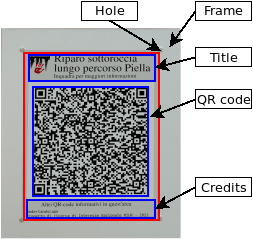
\includegraphics[width = 0.55 \linewidth]{figure/QR-code-legend.png}
	\label{fig:qrcodelegend}
}
\hfill
\subfloat[QR-tag content on a 5.5' screen]{
	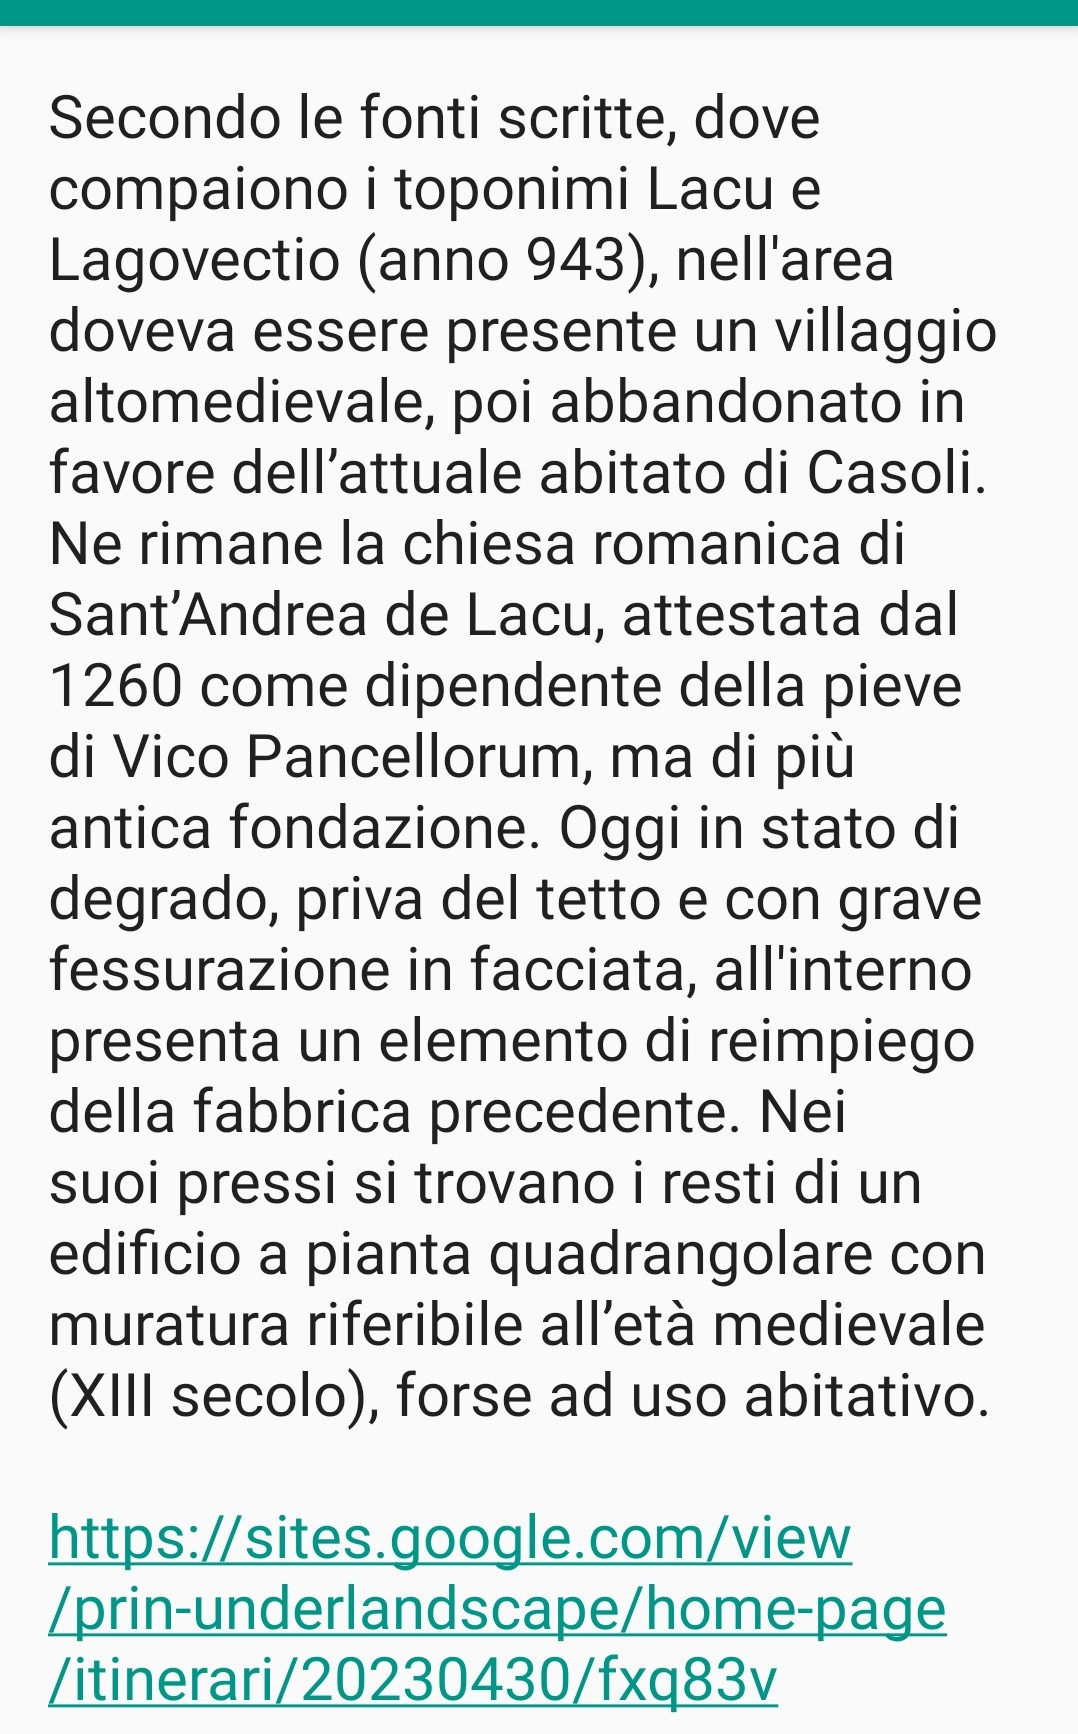
\includegraphics[width = 0.35 \linewidth]{figure/qr-code-content}
	\label{fig:qrcodecontent}
}
\caption{QR tag parts and content}
\end{figure}

\begin{figure}
\subfloat[Linked page: the map]{
	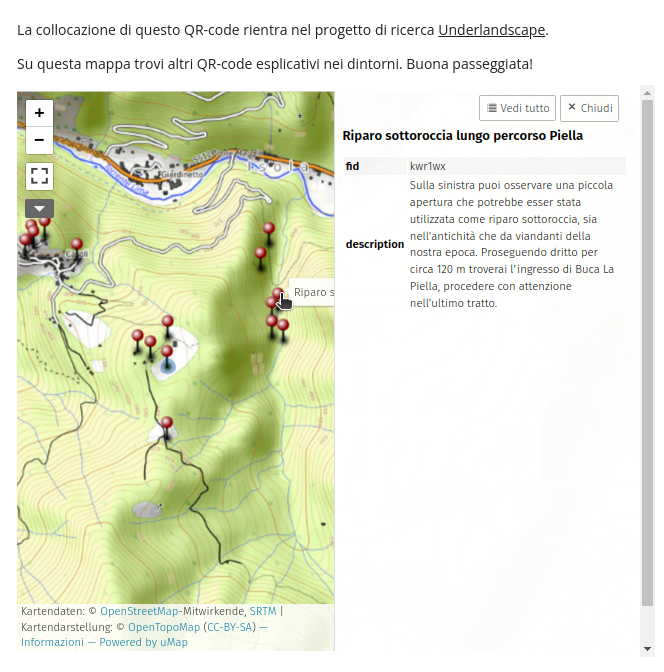
\includegraphics[width = 0.60 \linewidth]{figure/webpage-map}
	\label{fig:linkmap}
}
\subfloat[Linked page: survey form]{
	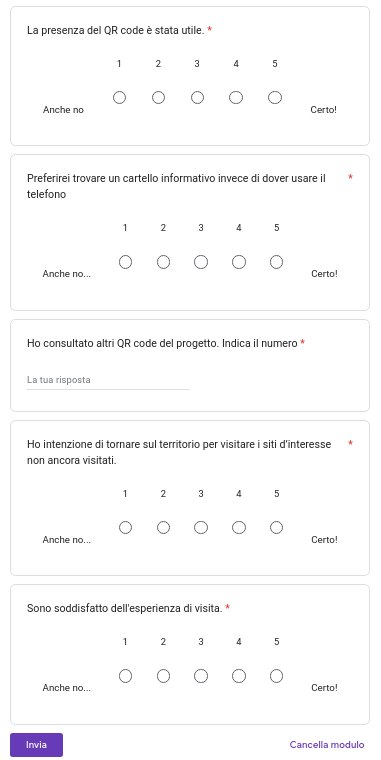
\includegraphics[width = 0.30 \linewidth]{figure/webpage-poll.png}
	\label{fig:linkpoll}
}
\caption{Content of the Web page linked to the URL in a QR tag}
\label{fig:webpage}
\end{figure}

\begin{table}
    \begin{tabular} {|>{\raggedright\arraybackslash}p{3cm}|l|l|l|l|}
        \hline 
        \textbf{Name} & \textbf{Long} & \textbf{Lat} & \textbf{URL Key} & \textbf{Length} \\ \hline
        Buca La Piella & 10.68361 & 44.03667 & t5ysrm & 476 \\ \hline
        Calendario celtico & 10.66985 & 44.03986 & my0kp8 & 484 \\ \hline
        Castello & 10.67062 & 44.04004 & 4l4r6y & 597 \\ \hline
        Chiesa dei SS. Donato e Andrea & 10.66947 & 44.03928 & lwtyx6 & 632 \\ \hline
        Iscrizione longobarda & 10.67244 & 44.03906 & 60m75s & 369 \\ \hline
        Lago di Casoli & 10.67761 & 44.03468 & xqjpbk & 369 \\ \hline
        Madonna di Castello & 10.66994 & 44.03960 & qlci89 & 395 \\ \hline
        Madonna di Col di Piano & 10.67760 & 44.03173 & 3w44wr & 414 \\ \hline
        Metato & 10.67764 & 44.03591 & sbgnl0 & 660 \\ \hline
        Sant'Andrea de Lacu & 10.67592 & 44.03530 & fxq83v & 657 \\ \hline
        Antro dell’Ugola & 10.68296 & 44.03871 & mprs0w & 226 \\ \hline
        Deviazione per Antro dell’Ugola & 10.68343 & 44.03971 & e4n2js & 88 \\ \hline
        Deviazione per Buca La Piella & 10.68427 & 44.03573 & hve4pj & 139 \\ \hline
        Deviazione per Sant’Andrea de Lacu & 10.67663 & 44.03507 & 13uav3 & 200 \\ \hline
        Ingresso Buca La Piella & 10.68358 & 44.03592 & 5ahvp8 & 190 \\ \hline
        Riparo sottoroccia lungo percorso Piella & 10.68401 & 44.03573 & kwr1wx & 286 \\    \hline
    \end{tabular}
\caption{The QR-tags placed around \emph{Casoli} . The URL key is a random code that appears on the web page linked to the QR code. The Length refers to the description in the QR tag and is in characters. \label{tab:qrtags}}
\end{table}

The production process of a series of tags has also been investigated to streamline the task and use only basic Information Technology skills.

The master document is a \emph{GeoJSON} file describing the area and the tagged features: a GPS tracking application can be used to record an initial version of it during a recon.

The finalized master document contains a single \emph{GeoJSON} \emph{FeatureCollection} object containing one \emph{Feature} object for each tag. Each \emph{Feature} contains a \emph{Geometry} object of type \emph{Point}, and a \emph{properties} object with fields containing information needed to create the tag: the \emph{uid}, a random string of six lowercase letters used to produce the associated URL, the \emph{title} printed on the tag, and the text encoded in the QR code (see table \ref{code:geojson}) where part of the {\em description} field is omitted. The \emph{properties} are also shown on the UMap map. 

Editing the basic map to fill-in the QR-code content and the other fields does not require technical skills since the tools integrated into the UMap user interface already fit the purpose (see figure \ref{fig:umap-editing}). The resulting geojson object for a tagged feature is shown in figure \ref{fig:geojson-sample}.

The master document is rendered by UMap on the page linked to the tags (as in figure \ref{fig:linkmap}).

\begin{figure}
\subfloat[Editing a feature associated with a QR-tag in UMap]{
	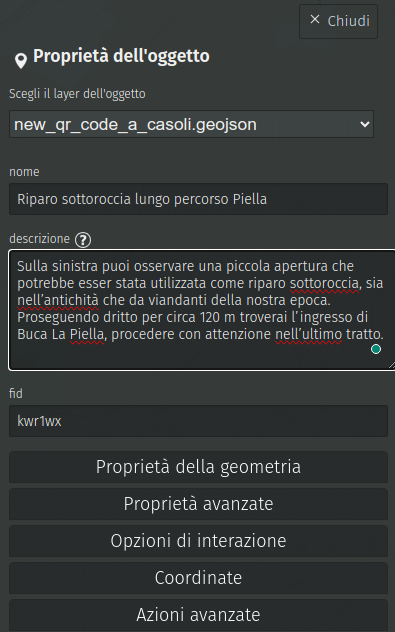
\includegraphics[width = 0.35 \linewidth]{figure/umap-editing.png}
	\label{fig:umap-editing}
}
\hfill
\subfloat[GeoJSON \emph{Object} representing the same the feature]{
	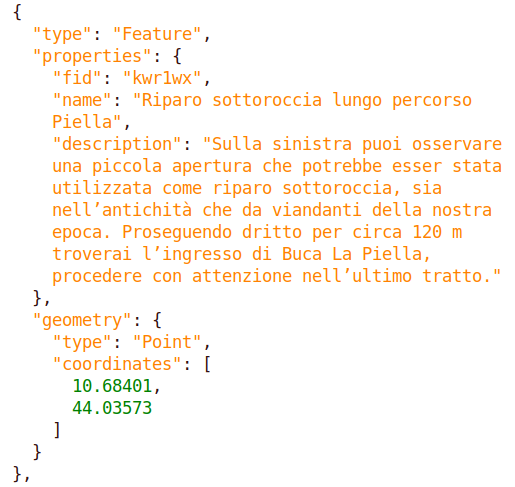
\includegraphics[width = 0.60 \linewidth]{figure/geojson-sample.png}
	\label{fig:geojson-sample}
}
\caption{Editing the GeoJSON with uMap editor. The resulting file is automatically converted into printable QR-tags}
\label{fig:editing}
\end{figure}

A \emph{Bash} script running on a Linux system makes straightforward the conversion of the GeoJSON file into a printable array of QR tags. The code, a total of 90 source lines written in Bash and Python taking advantage of the ogr2ogr and qrencode commands, is on GitHub \citeWeb{github-qr}.

\section{Results and discussion \label{sec:results}}

Our point is to illustrate a methodology to improve the touristic offer of a site that is not specific to a use case, but applicable to a broad range of frameworks. The methodology must be sustainable in the broader sense: social, environmental, and financial.

We applied the methodology to a small-scale example: a signage system addressing the guidance of visitors in a rural area with a cultural heritage to be protected and valorized at the same time.

Firstly we evaluated the aspects of interest of the site, and we found natural formations and human artifacts tracing back to the Paleolithic Era. Other relevant aspects are that the site is not included in mass tourism circuits but is not far from them. The area is exposed to depopulation due to the shortage of productive activities.

To preserve the native social and financial framework we do not aim at mass tourism. Instead, we target a motivated, non-casual visitor, and devise potential reasons for its visit. We found many of them: a not easily accessible cave inhabited since pre-history, a village with historical buildings, and nearby architecture dating back to the Middle Ages.

We investigated the task of guiding the visitor and telling the history of the place with inexpensive and non-intrusive techniques. The proposed solution consists of a dozen QR tags placed at key locations. The total cost of the tags amounts to a few Euros for the printing service, although finding a shop with an appropriate printing device may be difficult. The impact on the environment is extremely limited, as shown in figure \ref{fig:TagPlacement}.

\begin{figure}
\subfloat[A tag secured to a tree near a shelter]{
	\includegraphics[width = 0.33 \linewidth]{figure/Riparo1-070623-cut.jpg}
	\label{fig:TagOnTree}
}
\hfill
\subfloat[Google Earth view of the surroundings of the tag. The map is north-oriented, and shows  the village of \emph{Casoli}  in the left-high corner]{
	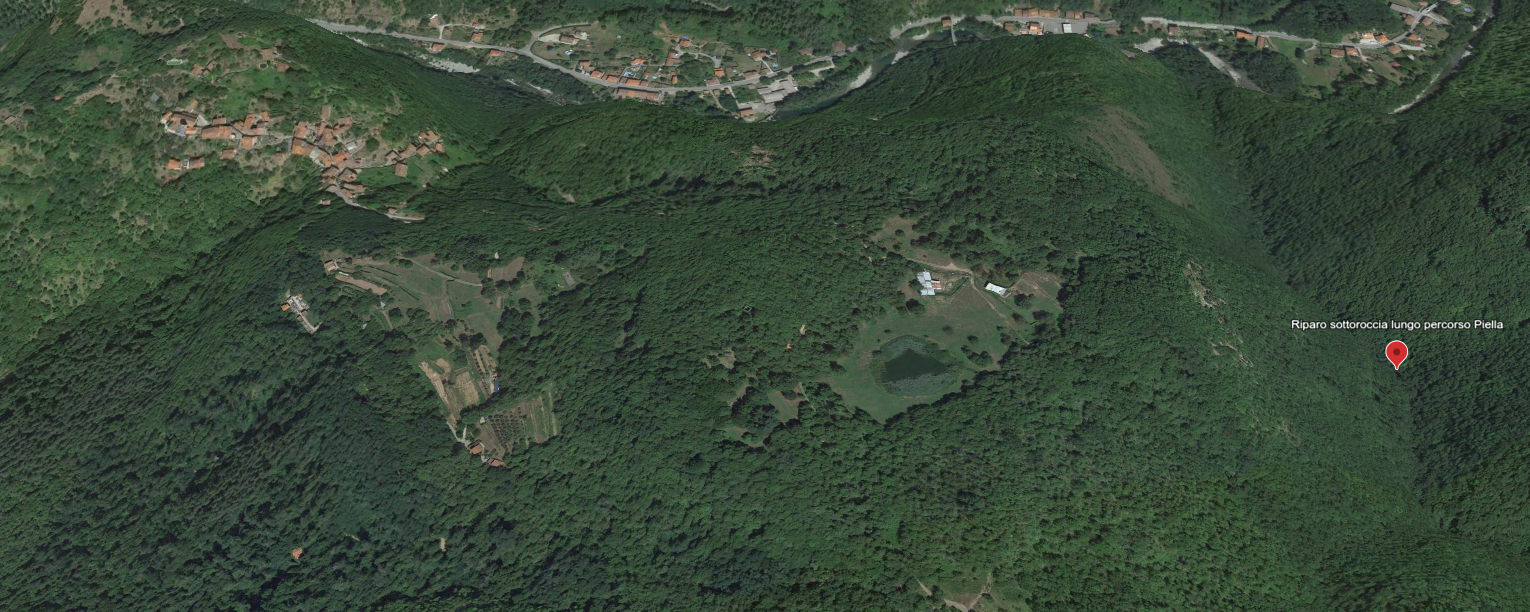
\includegraphics[width = 0.62 \linewidth]{figure/GoogleEarth.png}
	\label{fig:GoogleEarth}
}
\caption{Tag placement at different scales}
\label{fig:TagPlacement}
\end{figure}

The preparation of the signage requires a solid knowledge of the site. This demanded consulting historical documents, assessing the touristic vocation of the area, and two on-site surveys.

On the technical side, the proposed signage provides a benchmark difficult to improve in terms of environmental impact and cost, but its {\em performance} is difficult to evaluate.

One performance index might be the number of times a given tag is scanned. Indeed, we recorded several hits to the URLs in the QR tags, but their number and the way they are collected are not appropriate to form a statistic of their utilization. One reason is the fact that the use of the tag is not always associated with a hit, and vice-versa.

The reactions we collected by interviewing local stakeholders are positive, which gives us the impression that the initiative is respectful and consistent with the social and economic framework. The measurement of the efficacy in financial terms is beyond the scope of this paper, but it has to be said that the aim of this work is to provide assistance and improve the experience of actual visitors, not to multiply their number.

Although we are satisfied that the solution complies with the sustainability principles that inspired this work, we identified two issues that indicate directions for future research:

\begin{itemize}
    \item The balance between visual impact and effectiveness is critical. The current dimension of the tag is such that the visual impact is limited, but this negatively affects its efficacy: it is easy to miss a tag containing possibly relevant information;
    \item Monitoring visitor's activity, like the frequency of visits of a given tag, or the sequencing of visited tags, which may be of interest for managing the site, depends on user motivation.
\end{itemize}

Trading off cost and simplicity for effectiveness and measurability there are solutions, based, for instance, on Bluetooth communication or dedicated applications, that may improve such aspects.

\section{Conclusions}

Like any other productive activity, tourism is exposed to being unsustainable, damaging the very resources that allow it. To avoid heavy drawbacks the design of the activity has to consider the complex framework where it will operate, and the word used to indicate this is \emph{holistic}, and it is extremely difficult to put into practice. A methodology made of examples and guidelines simplifies the task.

This paper is a step in this direction. We address a common problem, that of providing the visitor with directions in an area not reached by mass tourism, with the aim of acquiring the financial resources for its survival while preserving its distinguishing traits.

We show how a balanced use of technology may help in the task, with a process that is necessarily multidisciplinary, joining skills coming from the diverse domains: sociology, economics, humanities and technical. The paper demonstrates how their interplay brings ad-hoc results targeting sustainability and efficacy.

The resulting implementation is original in the literature, and minimalistic in its deployment. The detailed description enables its reuse as a starting point in future initiatives.

The discussion regarding the deployed experiment indicates directions for future investigation on the technical side. For instance, the availability of non-intrusive long-range devices that send a message whenever sensing a presence might improve signals discoverability. The Bluetooth Low Evergy technology goes in that direction, but hidden tags with BLE and energy harvesting would have broken the economy constraints.

From a different point of view, the lack of discoverability suggests a recreational scenario inspired by Geocaching® and Pokemon-GO®.

In conclusion, more sustainable solutions to old problems exist and are reachable melting technology and humanities. Policy-makers are crucial in the development and monitoring of sustainable measures. This is especially important in the tourism industry where sustainability is a multifaceted topic that includes resident ecosystem resilience and regeneration efforts by both policy-makers and private tour operators.

%This section may be divided by subheadings. It should provide a concise and precise description of the experimental results, their interpretation as well as the experimental conclusions that can be drawn.
%\subsection{Subsection}
%\subsubsection{Subsubsection}

%Bulleted lists look like this:
%\begin{itemize}
%\item	First bullet;
%\item	Second bullet;
%\item	Third bullet.
%\end{itemize}

%Numbered lists can be added as follows:
%\begin{enumerate}
%\item	First item; 
%\item	Second item;
%\item	Third item.
%\end{enumerate}

%The text continues here. 
%
%\subsection{Figures, Tables, and Schemes}
%
%All figures and tables should be cited in the main text as Figure~\ref{fig1}, Table~\ref{tab1}, etc.
%
%\begin{figure}[H]
%
\includegraphics[width=10.5 cm]{Definitions/logo-mdpi}
%\caption{This is a figure. Schemes follow the same formatting. If there are multiple panels, they should be listed as: (\textbf{a}) Description of what is contained in the first panel. (\textbf{b}) Description of what is contained in the second panel. Figures should be placed in the main text near the first time they are cited. A caption on a single line should be centered.\label{fig1}}
%\end{figure}   
%\unskip
%
%\begin{table}[H] 
%\caption{This is a table caption. Tables should be placed in the main text near to the first time they are~cited.\label{tab1}}
%\newcolumntype{C}{>{\centering\arraybackslash}X}
%\begin{tabularx}{\textwidth}{CCC}
%\toprule
%\textbf{Title 1}	& \textbf{Title 2}	& \textbf{Title 3}\\
%\midrule
%Entry 1		& Data			& Data\\
%Entry 2		& Data			& Data \textsuperscript{1}\\
%\bottomrule
%\end{tabularx}
%\noindent{\footnotesize{\textsuperscript{1} Tables may have a footer.}}
%\end{table}
%
%The text continues here (Figure~\ref{fig2} and Table~\ref{tab2}).
%
%% Example of a figure that spans the whole page width. The same concept works for tables, too.
%\begin{figure}[H]
%\begin{adjustwidth}{-\extralength}{0cm}
%\centering
%
\includegraphics[width=15.5cm]{Definitions/logo-mdpi}
%\end{adjustwidth}
%\caption{This is a wide figure.\label{fig2}}
%\end{figure}  
%
%\begin{table}[H]
%\caption{This is a wide table.\label{tab2}}
%	\begin{adjustwidth}{-\extralength}{0cm}
%		\newcolumntype{C}{>{\centering\arraybackslash}X}
%		\begin{tabularx}{\fulllength}{CCCC}
%			\toprule
%			\textbf{Title 1}	& \textbf{Title 2}	& \textbf{Title 3}     & \textbf{Title 4}\\
%			\midrule
%\multirow[m]{3}{*}{Entry 1 *}	& Data			& Data			& Data\\
%			  	                   & Data			& Data			& Data\\
%			             	      & Data			& Data			& Data\\
%                   \midrule
%\multirow[m]{3}{*}{Entry 2}    & Data			& Data			& Data\\
%			  	                  & Data			& Data			& Data\\
%			             	     & Data			& Data			& Data\\
%                   \midrule
%\multirow[m]{3}{*}{Entry 3}    & Data			& Data			& Data\\
%			  	                 & Data			& Data			& Data\\
%			             	    & Data			& Data			& Data\\
%                  \midrule
%\multirow[m]{3}{*}{Entry 4}   & Data			& Data			& Data\\
%			  	                 & Data			& Data			& Data\\
%			             	    & Data			& Data			& Data\\
%			\bottomrule
%		\end{tabularx}
%	\end{adjustwidth}
%	\noindent{\footnotesize{* Tables may have a footer.}}
%\end{table}

%\begin{listing}[H]
%\caption{Title of the listing}
%\rule{\columnwidth}{1pt}
%\raggedright Text of the listing. In font size footnotesize, small, or normalsize. Preferred format: left aligned and single spaced. Preferred border format: top border line and bottom border line.
%\rule{\columnwidth}{1pt}
%\end{listing}

%Text.
%
%Text.
%
%\subsection{Formatting of Mathematical Components}
%
%This is the example 1 of equation:
%\begin{linenomath}
%\begin{equation}
%a = 1,
%\end{equation}
%\end{linenomath}
%the text following an equation need not be a new paragraph. Please punctuate equations as regular text.
%%% If the documentclass option "submit" is chosen, please insert a blank line before and after any math environment (equation and eqnarray environments). This ensures correct linenumbering. The blank line should be removed when the documentclass option is changed to "accept" because the text following an equation should not be a new paragraph.
%
%This is the example 2 of equation:
%\begin{adjustwidth}{-\extralength}{0cm}
%\begin{equation}
%a = b + c + d + e + f + g + h + i + j + k + l + m + n + o + p + q + r + s + t + u + v + w + x + y + z
%\end{equation}
%\end{adjustwidth}
%
%% Example of a page in landscape format (with table and table footnote).
%%\startlandscape
%%\begin{table}[H] %% Table in wide page
%%\caption{This is a very wide table.\label{tab3}}
%%	\begin{tabularx}{\textwidth}{CCCC}
%%		\toprule
%%		\textbf{Title 1}	& \textbf{Title 2}	& \textbf{Title 3}	& \textbf{Title 4}\\
%%		\midrule
%%		Entry 1		& Data			& Data			& This cell has some longer content that runs over two lines.\\
%%		Entry 2		& Data			& Data			& Data\textsuperscript{1}\\
%%		\bottomrule
%%	\end{tabularx}
%%	\begin{adjustwidth}{+\extralength}{0cm}
%%		\noindent\footnotesize{\textsuperscript{1} This is a table footnote.}
%%	\end{adjustwidth}
%%\end{table}
%%\finishlandscape
%
%
%Please punctuate equations as regular text. Theorem-type environments (including propositions, lemmas, corollaries etc.) can be formatted as follows:
%%% Example of a theorem:
%\begin{Theorem}
%Example text of a theorem.
%\end{Theorem}
%
%The text continues here. Proofs must be formatted as follows:
%
%%% Example of a proof:
%\begin{proof}[Proof of Theorem 1]
%Text of the proof. Note that the phrase ``of Theorem 1'' is optional if it is clear which theorem is being referred to.
%\end{proof}
%The text continues here.
%
%%%%%%%%%%%%%%%%%%%%%%%%%%%%%%%%%%%%%%%%%%%
%\section{Discussion}
%
%Authors should discuss the results and how they can be interpreted from the perspective of previous studies and of the working hypotheses. The findings and their implications should be discussed in the broadest context possible. Future research directions may also be highlighted.
%
%%%%%%%%%%%%%%%%%%%%%%%%%%%%%%%%%%%%%%%%%%%
%\section{Conclusions}
%
%This section is not mandatory, but can be added to the manuscript if the discussion is unusually long or complex.
%
%%%%%%%%%%%%%%%%%%%%%%%%%%%%%%%%%%%%%%%%%%%
%\section{Patents}
%
%This section is not mandatory, but may be added if there are patents resulting from the work reported in this manuscript.

%%%%%%%%%%%%%%%%%%%%%%%%%%%%%%%%%%%%%%%%%%
\vspace{6pt} 

%%%%%%%%%%%%%%%%%%%%%%%%%%%%%%%%%%%%%%%%%%
%% optional
%\supplementary{The following supporting information can be downloaded at:  \linksupplementary{s1}, Figure S1: title; Table S1: title; Video S1: title.}

% Only for the journal Methods and Protocols:
% If you wish to submit a video article, please do so with any other supplementary material.
% \supplementary{The following supporting information can be downloaded at: \linksupplementary{s1}, Figure S1: title; Table S1: title; Video S1: title. A supporting video article is available at doi: link.}

%%%%%%%%%%%%%%%%%%%%%%%%%%%%%%%%%%%%%%%%%%
\authorcontributions{For research articles with several authors, a short paragraph specifying their individual contributions must be provided. The following statements should be used ``Conceptualization, X.X. and Y.Y.; methodology, X.X.; software, X.X.; validation, X.X., Y.Y. and Z.Z.; formal analysis, X.X.; investigation, X.X.; resources, X.X.; data curation, X.X.; writing---original draft preparation, X.X.; writing---review and editing, X.X.; visualization, X.X.; supervision, X.X.; project administration, X.X.; funding acquisition, Y.Y. All authors have read and agreed to the published version of the manuscript.'', please turn to the  \href{http://img.mdpi.org/data/contributor-role-instruction.pdf}{CRediT taxonomy} for the term explanation. Authorship must be limited to those who have contributed substantially to the work~reported.}

\funding{Please add: ``This research received no external funding'' or ``This research was funded by NAME OF FUNDER grant number XXX.'' and  and ``The APC was funded by XXX''. Check carefully that the details given are accurate and use the standard spelling of funding agency names at \url{https://search.crossref.org/funding}, any errors may affect your future funding.}

\institutionalreview{In this section, you should add the Institutional Review Board Statement and approval number, if relevant to your study. You might choose to exclude this statement if the study did not require ethical approval. Please note that the Editorial Office might ask you for further information. Please add “The study was conducted in accordance with the Declaration of Helsinki, and approved by the Institutional Review Board (or Ethics Committee) of NAME OF INSTITUTE (protocol code XXX and date of approval).” for studies involving humans. OR “The animal study protocol was approved by the Institutional Review Board (or Ethics Committee) of NAME OF INSTITUTE (protocol code XXX and date of approval).” for studies involving animals. OR “Ethical review and approval were waived for this study due to REASON (please provide a detailed justification).” OR “Not applicable” for studies not involving humans or animals.}

\informedconsent{Any research article describing a study involving humans should contain this statement. Please add ``Informed consent was obtained from all subjects involved in the study.'' OR ``Patient consent was waived due to REASON (please provide a detailed justification).'' OR ``Not applicable'' for studies not involving humans. You might also choose to exclude this statement if the study did not involve humans.

Written informed consent for publication must be obtained from participating patients who can be identified (including by the patients themselves). Please state ``Written informed consent has been obtained from the patient(s) to publish this paper'' if applicable.}

\dataavailability{We encourage all authors of articles published in MDPI journals to share their research data. In this section, please provide details regarding where data supporting reported results can be found, including links to publicly archived datasets analyzed or generated during the study. Where no new data were created, or where data is unavailable due to privacy or ethical re-strictions, a statement is still required. Suggested Data Availability Statements are available in section “MDPI Research Data Policies” at \url{https://www.mdpi.com/ethics}.} 

\acknowledgments{In this section you can acknowledge any support given which is not covered by the author contribution or funding sections. This may include administrative and technical support, or donations in kind (e.g., materials used for experiments).}

\conflictsofinterest{Declare conflicts of interest or state ``The authors declare no conflict of interest.'' Authors must identify and declare any personal circumstances or interest that may be perceived as inappropriately influencing the representation or interpretation of reported research results. Any role of the funders in the design of the study; in the collection, analyses or interpretation of data; in the writing of the manuscript; or in the decision to publish the results must be declared in this section. If there is no role, please state ``The funders had no role in the design of the study; in the collection, analyses, or interpretation of data; in the writing of the manuscript; or in the decision to publish the~results''.} 

%%%%%%%%%%%%%%%%%%%%%%%%%%%%%%%%%%%%%%%%%%
%% Optional
\sampleavailability{Samples of the compounds ... are available from the authors.}

%% Only for journal Encyclopedia
%\entrylink{The Link to this entry published on the encyclopedia platform.}

\abbreviations{Abbreviations}{
The following abbreviations are used in this manuscript:\\

\noindent 
\begin{tabular}{@{}ll}
MDPI & Multidisciplinary Digital Publishing Institute\\
DOAJ & Directory of open access journals\\
TLA & Three letter acronym\\
LD & Linear dichroism
\end{tabular}
}

%%%%%%%%%%%%%%%%%%%%%%%%%%%%%%%%%%%%%%%%%%%
%%% Optional
%\appendixtitles{no} % Leave argument "no" if all appendix headings stay EMPTY (then no dot is printed after "Appendix A"). If the appendix sections contain a heading then change the argument to "yes".
%\appendixstart
%\appendix
%\section[\appendixname~\thesection]{}
%\subsection[\appendixname~\thesubsection]{}
%The appendix is an optional section that can contain details and data supplemental to the main text---for example, explanations of experimental details that would disrupt the flow of the main text but nonetheless remain crucial to understanding and reproducing the research shown; figures of replicates for experiments of which representative data are shown in the main text can be added here if brief, or as Supplementary Data. Mathematical proofs of results not central to the paper can be added as an appendix.
%
%\begin{table}[H] 
%\caption{This is a table caption.\label{tab5}}
%\newcolumntype{C}{>{\centering\arraybackslash}X}
%\begin{tabularx}{\textwidth}{CCC}
%\toprule
%\textbf{Title 1}	& \textbf{Title 2}	& \textbf{Title 3}\\
%\midrule
%Entry 1		& Data			& Data\\
%Entry 2		& Data			& Data\\
%\bottomrule
%\end{tabularx}
%\end{table}
%
%\section[\appendixname~\thesection]{}
%All appendix sections must be cited in the main text. In the appendices, Figures, Tables, etc. should be labeled, starting with ``A''---e.g., Figure A1, Figure A2, etc.
%
%%%%%%%%%%%%%%%%%%%%%%%%%%%%%%%%%%%%%%%%%%%
\begin{adjustwidth}{-\extralength}{0cm}
%%\printendnotes[custom] % Un-comment to print a list of endnotes

\reftitle{References}

% Please provide either the correct journal abbreviation (e.g. according to the “List of Title Word Abbreviations” http://www.issn.org/services/online-services/access-to-the-ltwa/) or the full name of the journal.
% Citations and References in Supplementary files are permitted provided that they also appear in the reference list here. 

%\nocite{*}
\bibliography{biblio/paper.bib}

\nociteWeb{*}
\bibliographystyleWeb{abbrv}
\bibliographyWeb{biblio/sitography.bib}

% If authors have biography, please use the format below
%\section*{Short Biography of Authors}
%\bio
%{\raisebox{-0.35cm}{\includegraphics[width=3.5cm,height=5.3cm,clip,keepaspectratio]{Definitions/author1.pdf}}}
%{\textbf{Firstname Lastname} Biography of first author}
%
%\bio
%{\raisebox{-0.35cm}{\includegraphics[width=3.5cm,height=5.3cm,clip,keepaspectratio]{Definitions/author2.jpg}}}
%{\textbf{Firstname Lastname} Biography of second author}

% For the MDPI journals use author-date citation, please follow the formatting guidelines on http://www.mdpi.com/authors/references
% To cite two works by the same author: \citeauthor{ref-journal-1a} (\citeyear{ref-journal-1a}, \citeyear{ref-journal-1b}). This produces: Whittaker (1967, 1975)
% To cite two works by the same author with specific pages: \citeauthor{ref-journal-3a} (\citeyear{ref-journal-3a}, p. 328; \citeyear{ref-journal-3b}, p.475). This produces: Wong (1999, p. 328; 2000, p. 475)

%%%%%%%%%%%%%%%%%%%%%%%%%%%%%%%%%%%%%%%%%%
%% for journal Sci
%\reviewreports{\\
%Reviewer 1 comments and authors’ response\\
%Reviewer 2 comments and authors’ response\\
%Reviewer 3 comments and authors’ response
%}
%%%%%%%%%%%%%%%%%%%%%%%%%%%%%%%%%%%%%%%%%%
\PublishersNote{}
\end{adjustwidth}

\end{document}

